%% This is the ctufit-thesis example file. It is used to produce theses
%% for submission to Czech Technical University, Faculty of Information Technology.
%%
%% Get the newest version from
%% https://gitlab.fit.cvut.cz/theses-templates/FITthesis-LaTeX
%%
%%
%% Copyright 2021, Eliska Sestakova and Ondrej Guth
%%
%% This work may be distributed and/or modified under the
%% conditions of the LaTeX Project Public Licenese, either version 1.3
%% of this license or (at your option) any later version.
%% The latest version of this license is in
%%  https://www.latex-project.org/lppl.txt
%% and version 1.3 or later is part of all distributions of LaTeX
%% version 2005/12/01 or later.
%%
%% This work has the LPPL maintenance status `maintained'.
%%
%% The current maintainer of this work is Ondrej Guth.
%% Contact ondrej.guth@fit.cvut.cz for bug reports.
%% Alternatively, submit bug reports into the tracker at
%% https://gitlab.fit.cvut.cz/theses-templates/FITthesis-LaTeX/issues
%%
%%

%%%%%%%%%%%%%%%%%%%%%%%%%%%%%%%%%%%%%%%%%
% CLASS OPTIONS
% language: czech/english/slovak
% thesis type: bachelor/master/dissertation
%%%%%%%%%%%%%%%%%%%%%%%%%%%%%%%%%%%%%%%%%
\documentclass[english,bachelor,unicode]{ctufit-thesis}

%%%%%%%%%%%%%%%%%%%%%%%%%%%%%%%%%%%%%%%%%
% ENGLISH PARAGRAPHS
%%%%%%%%%%%%%%%%%%%%%%%%%%%%%%%%%%%%%%%%%
\usepackage{parskip}
\setlength{\parindent}{0pt} % anglicke odstavce

%%%%%%%%%%%%%%%%%%%%%%%%%%%%%%%%%%%%%%%%%
% NUM OF SUBSECTIONS
%%%%%%%%%%%%%%%%%%%%%%%%%%%%%%%%%%%%%%%%%
\usepackage{titlesec}

\titleformat{\paragraph}
{\normalfont\normalsize\bfseries}{\theparagraph}{1em}{}
\titlespacing*{\paragraph}
{0pt}{3.25ex plus 1ex minus .2ex}{1.5ex plus .2ex}

\setcounter{secnumdepth}{2} % numbering sections
\setcounter{tocdepth}{2}
%%%%%%%%%%%%%%%%%%%%%%%%%%%%%%%%%%%%%%%%%
% VERSES
%%%%%%%%%%%%%%%%%%%%%%%%%%%%%%%%%%%%%%%%%
\usepackage{verse}

\newcommand{\su}[1]{\scansion{\smallerU}{#1}}
\newcommand{\sdash}[1]{\scansion{\smallerdash}{#1}}
\newcommand{\spipe}[1]{\scansion{\smallerpipe}{#1}}
\newcommand{\shash}[1]{\scansion{\smallerhash}{#1}}
\newcommand{\sS}[1]{\scansion{\smallerS}{#1}}
\newcommand{\sV}[1]{\scansion{\smallerV}{#1}}
\newcommand{\sW}[1]{\scansion{\smallerW}{#1}}

\newcommand{\scansion}[2]{%
  \begingroup
  \renewcommand{\arraystretch}{0}%
  \begin{tabular}[b]{@{}c@{}}
  \makebox[0pt]{#1}\\[0.5ex]
  \vphantom{T}#2
  \end{tabular}%
  \endgroup
}
\newcommand{\smallerU}{$\scriptstyle{U}$}
\newcommand{\smallerdash}{$\scriptstyle-$}
\newcommand{\smallerpipe}{$\scriptstyle|$}
\newcommand{\smallerhash}{$\scriptstyle\#$}
\newcommand{\smallerS}{$\scriptstyle{S}$}
\newcommand{\smallerV}{$\scriptstyle{V}$}
\newcommand{\smallerW}{$\scriptstyle{W}$}

\usepackage{ulem} % Underlining
\normalem

%%%%%%%%%%%%%%%%%%%%%%%%%%%%%%%%%%%%%%%%%
% TYPE ALGORITHMS
%%%%%%%%%%%%%%%%%%%%%%%%%%%%%%%%%%%%%%%%%
\usepackage{algorithm}
\usepackage{algorithmic}

%%%%%%%%%%%%%%%%%%%%%%%%%%%%%%%%%%%%%%%%%
% TABLES
%%%%%%%%%%%%%%%%%%%%%%%%%%%%%%%%%%%%%%%%%
\usepackage{makecell}
\usepackage{multirow}

%%%%%%%%%%%%%%%%%%%%%%%%%%%%%%%%%%
% FILL IN THIS INFORMATION
%%%%%%%%%%%%%%%%%%%%%%%%%%%%%%%%%%
\ctufittitle{Automatic poetic metre detection} % replace with the title of your thesis
\ctufitauthorfull{Kristýna Klesnilová} % replace with your full name (first name(s) and then family name(s) / surname(s)) including academic degrees
\ctufitauthorsurnames{Klesnilová} % replace with your surname(s) / family name(s)
\ctufitauthorgivennames{Kristýna} % replace with your first name(s) / given name(s)
\ctufitsupervisor{Ing.\,Karel Klouda,\,Ph.D.} % replace with name of your supervisor/advisor (include academic degrees)
\ctufitdepartment{Department of Applied Mathematics} % replace with the department of your defence
\ctufityear{2022} % replace with the year of your defence
\ctufitdeclarationplace{Prague} % replace with the place where you sign the declaration
\ctufitdeclarationdate{\today} % replace with the date of signature of the declaration

\ctufitabstractENG{This work is devoted to automatic metrical analysis of Czech syllabotonic verse metrically tagged inside a large poetic corpus -- the Corpus of Czech Verse. First, it reimplements the existing data-driven approach used by a program called KVĚTA. Later, it models the problem as a sequence tagging task and solves it using machine learning. The BiLSTM-CRF model is used, representing the current state of the art for many sequence tagging tasks. Many different input configurations are tested. In all experiments, the inputted syllables or word tokens are represented by Word2Vec word embeddings trained on training data. The results are evaluated by computing three different accuracies of the predictions: syllable-level accuracy, line-level accuracy, and poem-level accuracy. It is shown that using BiLSTM-CRF represents a great success. With the best input configurations, it produces better results than the KVĚTA reimplementation, with predictions achieving 99.61\% syllable accuracy, 98.86\% line accuracy, and 90.40\% poem accuracy. The most interesting finding is that the best results are obtained by inputting sequences representing whole poems instead of individual poem lines.}
\ctufitabstractCZE{Tato práce se zabývá automatickou metrickou analýzou českého sylabotonického verše, jenž je metricky otagován ve velkém korpusu básní – v Korpusu českého verše. Práce nejprve reimplementuje přístup založený na datech, který využívá program s názvem KVĚTA. Poté si metrickou analýzu namodeluje jako úlohu tagování sekvencí a řeší ji pomocí strojového učení. Je trénován model BiLSTM-CRF, který reprezentuje aktuálně nejlepší architekturu pro většinu klasických úloh tagování sekvencí. Je otestováno mnoho různých vstupních konfigurací. Ve všech experimentech jsou slabiky nebo tokeny slov na vstupu reprezentovány pomocí Word2Vec embeddingů natrénovaných na trénovacích datech. Výsledky jsou vyhodnoceny pomocí spočítání tří různých přesností predikce: přesnosti pro jednotlivé slabiky, přesnosti pro jednotlivé řádky básní a přesnosti pro celé básně. Je ukázáno, že použití modelu BiLSTM-CRF představuje velký úspěch. S nejlepšími vstupními konfiguracemi vrací BiLSTM-CRF lepší výsledky než reimplementace programu KVĚTA s~predikcemi dosahujícími 99.61\% přesnosti pro jednotlivé slabiky, 98.86\% přesnosti pro jednotlivé řádky básní a 90.40\% přesnosti pro celé básně. Nejzajímavější zjištění představuje fakt, že nejlepších výsledků je dosaženo pro vstupní sekvence reprezentují celé básně namísto jednotlivých řádků básní.}

% 5-12 slov
\ctufitkeywordsENG{automatic metrical analysis of verse, Czech syllabotonic verse, Corpus of Czech Verse, KVĚTA, BiLSTM-CRF, Word2Vec}
\ctufitkeywordsCZE{automatická metrická analýza verše, český sylabotonický verš, Korpus českého verše, KVĚTA, BiLSTM-CRF, Word2Vec}
%%%%%%%%%%%%%%%%%%%%%%%%%%%%%%%%%%
% END FILL IN
%%%%%%%%%%%%%%%%%%%%%%%%%%%%%%%%%%

%%%%%%%%%%%%%%%%%%%%%%%%%%%%%%%%%%
% CUSTOMIZATION of this template
% Skip this part or alter it if you know what you are doing.
%%%%%%%%%%%%%%%%%%%%%%%%%%%%%%%%%%

\RequirePackage{iftex}[2020/03/06]
\iftutex % XeLaTeX and LuaLaTeX
    \RequirePackage{ellipsis}[2020/05/22] %ellipsis workaround for XeLaTeX
\else
    \RequirePackage[utf8]{inputenc}[2018/08/11] %this file encoding
    \RequirePackage{lmodern}[2009/10/30] % vector flavor of Computer Modern font
\fi

% hyperlinks
\RequirePackage[pdfpagelayout=TwoPageRight,colorlinks=false,allcolors=decoration,pdfborder={0 0 0.1}]{hyperref}[2020-05-15]

% uncomment the following to hide all hyperlinks
% \RequirePackage[pdfpagelayout=TwoPageRight,hidelinks]{hyperref}[2020-05-15]

\RequirePackage{pdfpages}[2020/01/28]


%%%%%%%%%%%%%%%%%%%%%%%%%%%%%%%%%%
% CUSTOMIZATION of this template END
%%%%%%%%%%%%%%%%%%%%%%%%%%%%%%%%%%


%%%%%%%%%%%%%%%%%%%%%%
% DEMO CONTENTS SETTINGS
% You may choose to modify this part.
%%%%%%%%%%%%%%%%%%%%%%
\usepackage{dirtree}
\usepackage{lipsum,tikz}
\usepackage{csquotes}
\usepackage[style=iso-numeric]{biblatex}
\addbibresource{text/bib-database.bib}
\usepackage{listings} % typesetting of sources
\usepackage{minted} % typesetting of sources
\counterwithin{listing}{chapter}

%theorems, definitions, etc.
\theoremstyle{plain}
\newtheorem{theorem}{Věta}
\newtheorem{lemma}[theorem]{Tvrzení}
\newtheorem{corollary}[theorem]{Důsledek}
\newtheorem{proposition}[theorem]{Návrh}
\newtheorem{definition}[theorem]{Definice}
\theoremstyle{definition}
\newtheorem{example}[theorem]{Příklad}
\theoremstyle{remark}
\newtheorem{note}[theorem]{Poznámka}
\newtheorem*{note*}{Poznámka}
\newtheorem{remark}[theorem]{Pozorování}
\newtheorem*{remark*}{Pozorování}
\numberwithin{theorem}{chapter}
%theorems, definitions, etc. END
%%%%%%%%%%%%%%%%%%%%%%
% DEMO CONTENTS SETTINGS END
%%%%%%%%%%%%%%%%%%%%%%

\begin{document} 
\frontmatter\frontmatterinit % do not remove these two commands

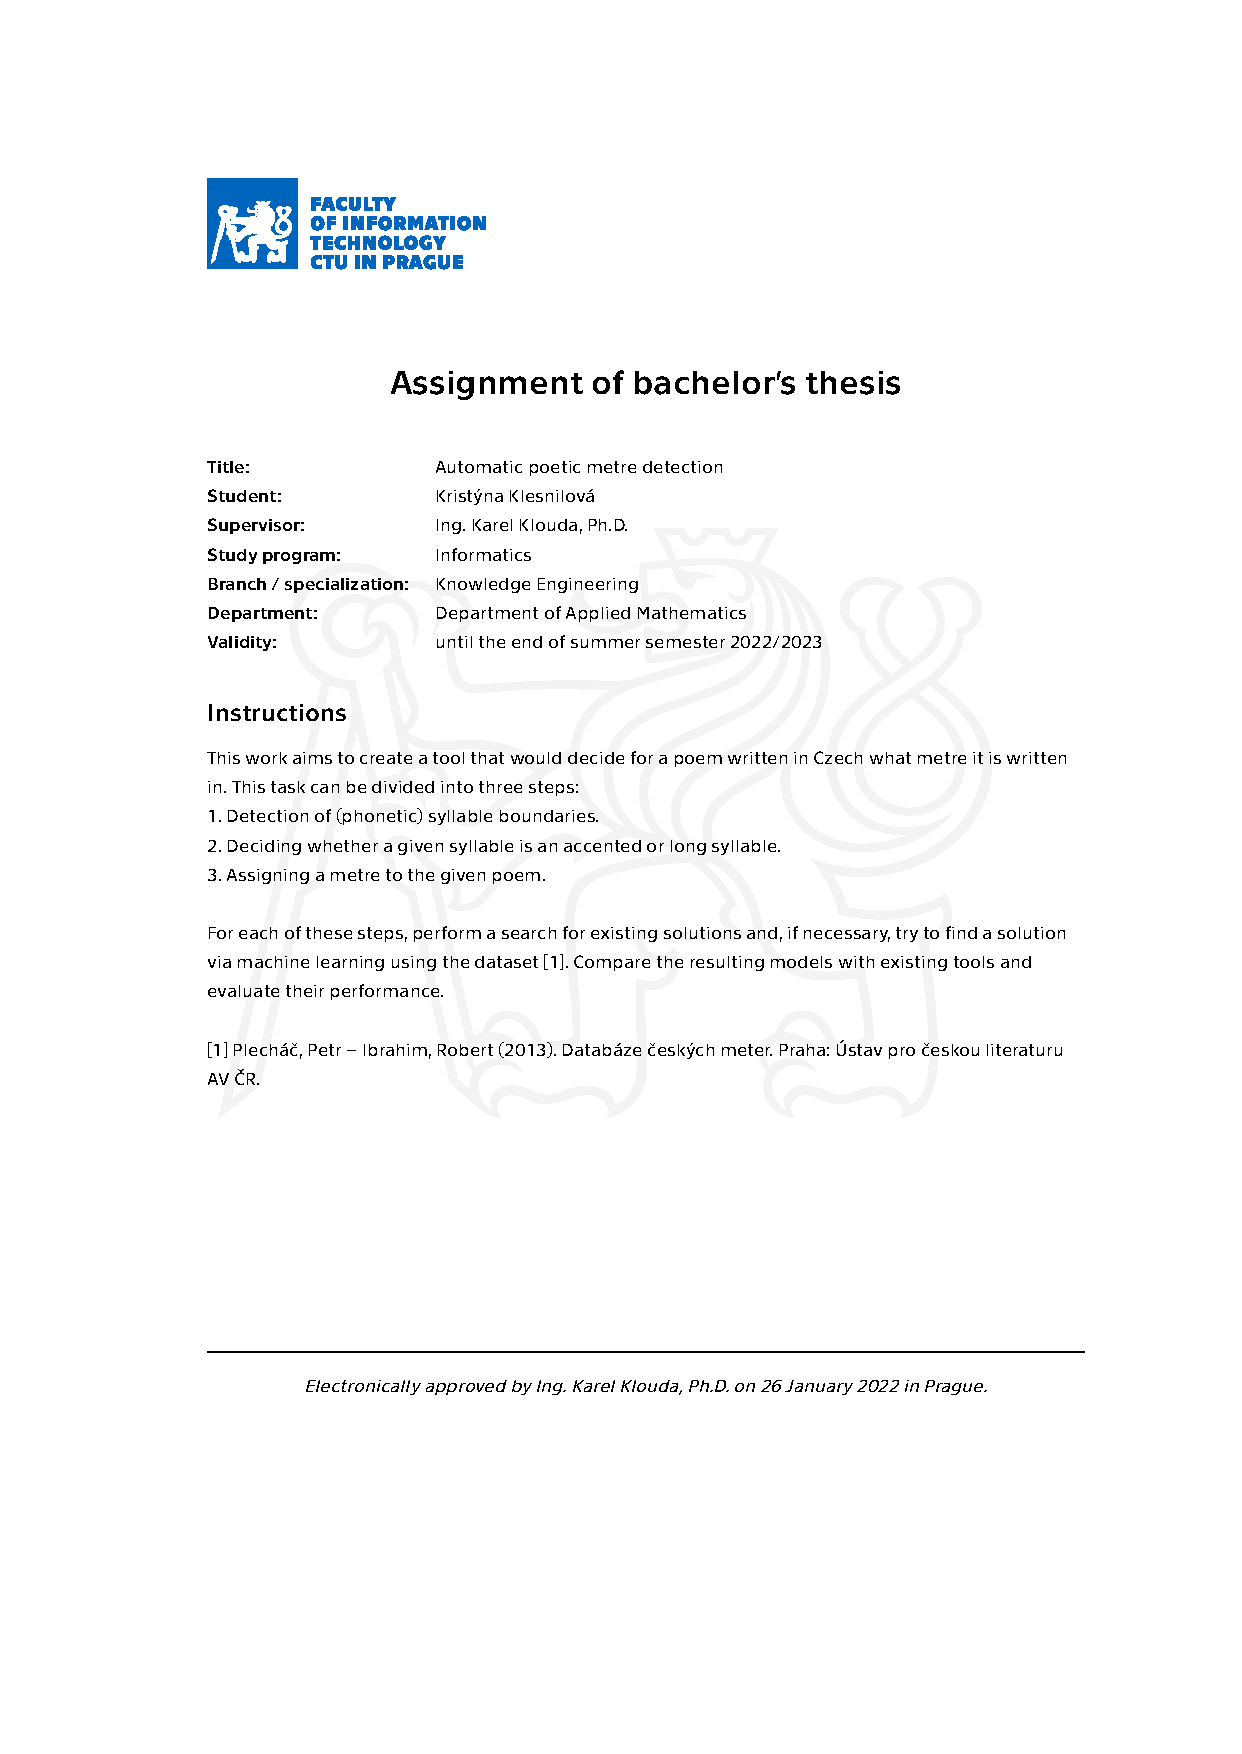
\includepdf{assignment-include.pdf} % replace that file with your thesis assignment provided by study office

\thispagestyle{empty}\cleardoublepage\maketitle % do not remove these three commands

\imprintpage % do not remove this command

\tableofcontents % do not remove this command
%%%%%%%%%%%%%%%%%%%%%%
% list of other contents: figures, tables, code listings, algorithms, etc.
% add/remove commands accordingly
%%%%%%%%%%%%%%%%%%%%%%
\listoffigures % list of figures
\begingroup
\let\clearpage\relax
\listoftables % list of tables
% \listoflistings % list of source code listings generated by the listings package
% \listoflistings % list of source code listings generated by the minted package
\endgroup
%%%%%%%%%%%%%%%%%%%%%%
% list of other contents END
%%%%%%%%%%%%%%%%%%%%%%

%%%%%%%%%%%%%%%%%%%
% ACKNOWLEDGMENT
% FILL IN / MODIFY
% This is a place to thank people for helping you. It is common to thank your supervisor.
%%%%%%%%%%%%%%%%%%%
\begin{acknowledgmentpage}
    In the first place, I would like to express sincere gratitude to my supervisor, Ing.\,Karel Klouda,\,Ph.D., for all his excellent advice and constant guidance in writing this thesis. Next, I would like to thank my family and friends for their support during my studies. Especially to all the amazing friends from CHS, who made my studies much more fun.
\end{acknowledgmentpage} 
%%%%%%%%%%%%%%%%%%%
% ACKNOWLEDGMENT END
%%%%%%%%%%%%%%%%%%%


%%%%%%%%%%%%%%%%%%%
% DECLARATION
% FILL IN / MODIFY
%%%%%%%%%%%%%%%%%%%
% INSTRUCTIONS
% ENG: choose one of approved texts of the declaration. DO NOT CREATE YOUR OWN. Find the approved texts at https://courses.fit.cvut.cz/SFE/download/index.html#_documents (document Declaration for FT in English)
% CZE/SLO: Vyberte jedno z fakultou schvalenych prohlaseni. NEVKLADEJTE VLASTNI TEXT. Schvalena prohlaseni najdete zde: https://courses.fit.cvut.cz/SZZ/dokumenty/index.html#_dokumenty (prohlášení do ZP)
\begin{declarationpage}
I hereby declare that the presented thesis is my own work and that I have cited all
sources of information in accordance with the Guideline for adhering to ethical
principles when elaborating an academic final thesis.

I acknowledge that my thesis is subject to the rights and obligations stipulated by the
Act No. 121/2000 Coll., the Copyright Act, as amended, in particular that the Czech
Technical University in Prague has the right to conclude a license agreement on the
utilization of this thesis as a school work under the provisions of Article 60 (1) of the Act.
\end{declarationpage}
%%%%%%%%%%%%%%%%%%%
% DECLARATION END
%%%%%%%%%%%%%%%%%%%

\printabstractpage % do not remove this command

%%%%%%%%%%%%%%%%%%%
% SUMMARY
% FILL IN / MODIFY
% OR REMOVE ENTIRELY (upon agreement with your supervisor)
% (appropriate to remove in most theses)
%%%%%%%%%%%%%%%%%%%
% \begin{summarypage}
% \section*{Summary section}

% \lipsum[1][1-8]

% \section*{Summary section}

% \lipsum[2][1-6]

% \section*{Summary section}

% \lipsum[3]

% \section*{Summary section}

% \lipsum[2]

% \section*{Summary section}

% \lipsum[1][1-8] Lorem lorem lorem.
% \end{summarypage}
%%%%%%%%%%%%%%%%%%%
% SUMMARY END
%%%%%%%%%%%%%%%%%%%

%%%%%%%%%%%%%%%%%%%
% ABBREVIATIONS
% FILL IN / MODIFY
% OR REMOVE ENTIRELY
% List the abbreviations in lexicography order.
%%%%%%%%%%%%%%%%%%%
\chapter{List of abbreviations}
	
\begin{tabular}{rl}
POS & Part of speech\\
NER & Named entity recognition\\
RNN & Recurrent neural network\\
LSTM & Long short-term memory\\
BiLSTM & Bidirectional LSTM\\
CRF & Conditional random fields\\
LSTM-CRF & LSTM network with a CRF layer\\
BiLSTM-CRF & Bidirectional LSTM network with a CRF layer\\
CNN & Convolutional neural network\\
SGD & Stochastic gradient descent\\
HMM & Hidden Markov model\\
MPP & Monosyllabic preposition proper
\end{tabular}
%%%%%%%%%%%%%%%%%%%
% ABBREVIATIONS END
%%%%%%%%%%%%%%%%%%%

\mainmatter\mainmatterinit % do not remove these two commands

%%%%%%%%%%%%%%%%%%%
% THE THESIS
% MODIFY ANYTHING BELOW THIS LINE
%%%%%%%%%%%%%%%%%%%

% Do not forget to include Introduction
%---------------------------------------------------------------
\chapter*{Introduction}\addcontentsline{toc}{chapter}{Introduction}\markboth{Introduction}{Introduction}
%---------------------------------------------------------------
\setcounter{page}{1}

Metrical analysis of verse is an important versology task that consists of analysing a poem and deciding in which metre it is written. This task is challenging not only because of the complexity of its subtasks (splitting a word into syllables, deciding whether a syllable is accented or long \ldots) but also due to the fact that poets -- as all artists -- tend to be creative and do not always follow the metrical norms precisely. Therefore, all algorithms and proposed approaches must take these \enquote{creative mistakes} into account.

In the past, metrical analysis had to be performed only algorithmically using rule-based approaches. Nowadays, there exist large corpora containing many semi-automatically tagged poems, and thanks to that, data-driven approaches are possible. In this work, one such corpus is used -- the Corpus of Czech Verse~\cite{CorpusCzechVerse}. This work reimplements the statistical approach to the metrical analysis of Czech syllabotonic verse as performed within the Czech verse processing system KVĚTA, which was developed by the authors of the Corpus of Czech Verse. Afterwards, the task is modelled as a sequence tagging task, and further experiments are performed using a state-of-the-art machine learning approach -- the BiLSTM-CRF model for sequence tagging. The use of this model has been recently proposed by versology researchers~\cite{ComparisonFeatureBasedNeualScansion}, but it has not yet been tested on the Czech syllabotonic verses inside the Corpus of Czech Verse.

\section*{Motivation}
The results of this thesis will be beneficial to versology researchers, as the BiLSTM-CRF model is used for the first time with Czech syllabotonic verse. If this work proposes some new input configurations for the BiLSTM-CRF model, the configurations may be beneficial even for researchers working with verses written in other languages.

\section*{Thesis structure}
This work begins with a theoretical background. It introduces necessary concepts from the theory of verse and machine learning (Chapters~\ref{chap:verse-theory} and~\ref{chap:ml-theory}), describes the Corpus of Czech Verse (Chapter~\ref{chap:ccv}) and presents the metrical analysis pipeline with all its subtasks and possible approaches to solve them (Chapter~\ref{chap:metrical-analysis}). Later, it continues with a practical part, where the reimplementation of the KVĚTA program and training of the BiLSTM-CRF model with various input configurations are described (Chapter~\ref{chap:implementation}). Finally, the obtained results are presented and discussed (Chapter~\ref{chap:results}).

\section*{Objectives}
The theoretical part of this work aims to build common ground and introduce the reader to the concepts of verse and machine learning theory used in this thesis. Furthermore, it intends to present the structure and contents of the Corpus of Czech Verse, the metrical tagging pipeline with all its subtasks, and the existing approaches to solve this task.

The objective of the practical part is to reimplement the KVĚTA data-driven approach and train the BiLSTM-CRF sequence tagging model. For the BiLSTM-CRF, the goal is to propose various input configurations that may be beneficial to the model and to test all of them. Based on the obtained results, the aim is to decide whether using the BiLSTM-CRF model for the metrical tagging of Czech syllabotonic verse is successful and has some benefits over using the KVĚTA approach.
\chapter{Verse theory}\label{chap:verse-theory}

\begin{chapterabstract}
This chapter introduces essential concepts from verse theory that are used throughout this thesis and are vital for a better understanding of the rest of this work.
\end{chapterabstract}

\section{Poem structure}

\subsection{Verse}
Poetry is written in verse. A common misconception is that one verse is equivalent to one line in a poem. That is not true in all cases. The verse does not have to end with a line end, but it can be spread across multiple lines. This often occurs, for example, inside dialogues in verse dramas. When a verse does not end with a line end, it is called an \emph{enjambement}.~\cite{TeorieLiteraturySS}

For an example of an enjambement, see Figure~\ref{fig:enjambement}.

\begin{figure}[htpb]
    \centering
    \settowidth{\versewidth}{se těsně k ní, vytáhne z haleny}
    \begin{verse}[\versewidth]
    Dí paní domu; dítě přiblíží\\
    se těsně k ní, vytáhne z haleny\\
    list složený...
    \end{verse}
    \caption[Enjambement]{Enjambement~\cite{UvodTeorieVerse}}\label{fig:enjambement}
\end{figure}

\subsection{Strophe}
Verses inside a poem can be organised into strophes. A strophe is a group of verses that form a semantic unit and tend to be graphically separated. The strophe is then repeated throughout the poem with similar or almost similar properties (same number of verses, same metrical or rhyme scheme). Strophes tend to contain 2--14 verses -- strophes with an even number of verses are more common. When shorter and longer verses alternate in a strophe, then usually in such an order that a longer verse comes before a shorter one. The last verse of a strophe tends to be shorter or less rhythmically regular.~\cite{TeorieLiteraturySS} Some strophes even have special names assigned to them, for example, \emph{the Sapphic stanza}, \emph{the Alcaic stanza}, \emph{the Second Asclepiad stanza}, or \emph{the Fourth Asclepiad stanza}.~\cite{UvodTeorieVerse}

\subsection{Paragraph (Stanza)}
However, in many poems, groups of verses can be encountered that are graphically separated; nevertheless, their internal organisation lacks any regularity. These are not called strophes but paragraphs (stanzas).~\cite{TeorieLiteraturySS}

\section{Versification systems}
This section introduces four important versification systems -- \emph{syllabic}, \emph{quantitative}, \emph{tonic}, and \emph{syllabotonic} -- along with the different approaches towards versification. However, only syllabotonic versification will be further discussed in the rest of this work, as within the Corpus of Czech Verse, metres are assigned only to syllabotonic verses.~\cite{CorpusCzechVerse}

\subsection{Syllabic versification system}
Probably the oldest versification system used in Indo-European languages, syllabic, distinguishes verses only by the number of syllables they contain. Syllabic versification does not care whether the syllables are accented or long, the only important thing is their number.~\cite{UvodTeorieVerse} In Czech poetry, the syllabic verse was used until the end of the 18\textsuperscript{th} century. After that, it appeared only episodically, especially in folk poetry.~\cite{TeorieLiteraturySS}

In the excerpt from the poem \emph{Co Bůh? Člověk?} by Fridrich Bridel (see Figure~\ref{fig:syllabic-versification}), no regularity can be found in the alternation of long and short syllables or the accented and non-accented syllables. However, it can be noted that 7-syllable and 8-syllable verses regularly alternate and verses with the same number of syllables rhyme. Therefore, it represents a syllabic versification.~\cite{TeorieLiteraturySS}

\begin{figure}[htpb]
    \centering
    \settowidth{\versewidth}{stro|jí | se | vše|cko | k lí|tá|ní. \textsubscript{(8 syll.)}}
    \begin{verse}[\versewidth]
    Ja|ký | boj? | Ja|ké | hnu|tí? \textsubscript{(7 syll.)}\\
    mně | vstu|pu|jí | na | myš|le|ní? \textsubscript{(8 syll.)}\\
    Mám|-li | snad | za|hy|nou|ti? \textsubscript{(7 syll.)}\\
    Či|ji | mdlé | při|ro|ze|ní. \textsubscript{(7 syll.)}\\
    Což | to? | Věc | vel|mi | rych|lá, \textsubscript{(7 syll.)}\\
    a|neb | jest|-li | ňá|ké | zdá|ní, \textsubscript{(8 syll.)}\\
    ros|tou | mně | ja|kás | kří|dla, \textsubscript{(7 syll.)}\\
    stro|jí | se | vše|cko | k lí|tá|ní. \textsubscript{(8 syll.)}\\
    \end{verse}
    \caption{Syllabic versification}\label{fig:syllabic-versification}
\end{figure}

\subsection{Quantitative versification system}
The quantitative versification system differentiates between long and short syllables. The long and short syllables are annotated according to the rules that take diphthongs, vocals, and syllable-forming consonants into account. Quantitative verse can be found in Greek and Roman poetry. In Czech poetry, it was used mainly in the 16\textsuperscript{th} century and then shortly in the 1920s.

In the quantitative versification system, a syllable can be long by nature or long by position. Syllable long by nature contains a long vocal or a diphthong. Meanwhile, a syllable long by position contains either a short vocal or a syllable-forming consonant \emph{l} or \emph{r}. This short vocal or syllable-forming consonant is followed by two or more consonants (not necessarily belonging to the same syllable). On the other hand, when a syllable contains a short vocal or a syllable-forming consonant followed by only one consonant, the syllable is classified as short.

When a syllable contains a short vocal or a syllable-forming consonant followed by exactly two consonants and one of the two consonants is \emph{l}, \emph{r}, \emph{ř}, \emph{m} or \emph{n}, the syllable can be long or short depending on the context.

In the passage from the poem \emph{Noční bdění} by I. V. Šimko (see Figure~\ref{fig:quantitative-versification}), all long syllables occupy an odd position -- except for the second position in the last verse and the final positions in all verses except the last one. The final position in verse represented a common exception and could be occupied by both long and short syllables. Therefore, the poem is classified as quantitative.~\cite{TeorieLiteraturySS}

\begin{figure}[htpb]
    \centering
    \settowidth{\versewidth}{\uline{a} | v le|\uline{sích} | zpě|\uline{vák} | mi|\uline{lost}|\uline{ný}}
    \begin{verse}[\versewidth]
    \uline{sen} | mi|\uline{lý} | po|\uline{koj}|ně | \uline{lí}|\uline{tá},\\
    \uline{a} | v le|\uline{sích} | zpě|\uline{vák} | mi|\uline{lost}|\uline{ný}\\
    \uline{s pří}|ro|\uline{dou} | ce|\uline{lou} | spo|\uline{čí}|\uline{vá}:\\
    \uline{teh}|dy | \uline{já} | se | \uline{mar}|ně | \uline{trá}|\uline{pím}\\
    \uline{blou}|\uline{dě} | \uline{v há}|ji | \uline{až} | do | \uline{rá}|na\\
    \end{verse}
    \caption[Quantitative versification]{Quantitative versification (long syllables are underlined)}\label{fig:quantitative-versification}
\end{figure}

\subsection{Tonic versification system}
Tonic versification was the second most important versification system in medieval Europe. The tonic verse normalises the number of accents in a line. Usage in Czech poetry is very rare, oftentimes readers confuse it with free verse~\cite{UvodTeorieVerse} (verse without a metrical norm~\cite{TeorieLiteraturySS}).

In the example of a tonic poetic text (see Figure~\ref{fig:tonic-versification}), every verse has exactly four accents, but the syllable counts differ.~\cite{UvodTeorieVerse}

\begin{figure}[htpb]
    \centering
    \settowidth{\versewidth}{A | \uline{vrá}|til | se | \uline{Mu}|ro|mec | \uline{k dob}|ré|mu | \uline{mlád}|ci, \textsubscript{(4 acc., 12 syll.)}}
    \begin{verse}[\versewidth]
    A | \uline{vrá}|til | se | \uline{Mu}|ro|mec | \uline{k dob}|ré|mu | \uline{mlád}|ci, \textsubscript{(4 acc., 12 syll.)}\\
    \uline{K mlád}|ci | \uline{to}|mu | \uline{dob}|ré|mu, | \uline{u}|bi|té|mu; \textsubscript{(4 acc., 11 syll.)}\\
    On | \uline{vy}|ko|pal | \uline{hrob} | \uline{v ší}|rém | \uline{po}|li, \textsubscript{(4 acc., 9 syll.)}\\
    \uline{Do} | to|ho | \uline{hro}|bu | \uline{tě}|lo | \uline{po}|lo|žil \textsubscript{(4 acc., 10 syll.)}\\
    \end{verse}
    \caption[Tonic versification]{Tonic versification (accented syllables are underlined)}\label{fig:tonic-versification}
\end{figure}

\subsection{Syllabotonic versification system}
Syllabotonic versification combines syllabic and tonic versification considering not only the number of syllables but also whether they are accented or not.~\cite{UvodTeorieVerse}

In the excerpt from the poem \emph{U studánky} by Jan Neruda (see Figure~\ref{fig:syllabotonic-versification}), every accented syllable, except the second syllable in the fourth verse, occupies an odd position in verse. Furthermore, every verse has exactly eight syllables. Therefore, syllabotonic versification is used.~\cite{TeorieLiteraturySS}

\begin{figure}[htpb]
    \centering
    \settowidth{\versewidth}{\uline{ble}|dé | \uline{ja}|ko | \uline{ru}|báš | \uline{z kmen}|tu. \textsubscript{(8 syll.)}}
    \begin{verse}[\versewidth]
    \uline{U} | stu|dá|nky | \uline{sto}|jí | \uline{děv}|če, \textsubscript{(8 syll.)}\\
    \uline{mla}|dé | \uline{ja}|ko | \uline{strů}|mek | \uline{mla}|dý, \textsubscript{(8 syll.)}\\
    \uline{ble}|dé | \uline{ja}|ko | \uline{ru}|báš | \uline{z kmen}|tu. \textsubscript{(8 syll.)}\\
    A | \uline{na} | ne|bi | \uline{bí}|lý | \uline{mě}|síc, \textsubscript{(8 syll.)}\\
    \uline{ko}|lem | \uline{ně}|ho | \uline{vod}|ní | \uline{ko}|lo \textsubscript{(8 syll.)}\\
    \uline{jak} | by | \uline{ze} | stu|dá|nky | \uline{hle}|děl. \textsubscript{(8 syll.)}\\
    \end{verse}
    \caption[Syllabotonic versification]{Syllabotonic versification (accented syllables are underlined)}\label{fig:syllabotonic-versification}
\end{figure}

In the rest of this work, the Czech syllabotonic verse will be discussed.

\section{Metrical analysis properties}
When performing a metrical analysis of a poem, various properties of the verse can be examined.

\subsection{Foot}
The basic metrical unit of a verse is called a foot. In the syllabotonic verse, it represents a group of at least two syllables that is repeated regularly throughout the verse. One foot consists of strong and weak positions. Strong positions are labelled with \textbf{S}, and weak positions are labelled with \textbf{W}. If there are two weak positions within a foot, the first is labelled using \textbf{V}. Table~\ref{tab:czech-syllabotonic-feet} presents all types of feet that can be encountered within the Czech syllabotonic verse.~\cite{UvodTeorieVerse}

\begin{table}[htpb]
\caption[Czech syllabotonic verse feet]{Czech syllabotonic verse feet (positions inside brackets can be omitted)}\label{tab:czech-syllabotonic-feet}
\centering
\begin{tabular}{|c||l|}\hline
    Foot & Feet pattern\\\hline\hline
    Iamb & W\textsubscript{0} S\textsubscript{1} W\textsubscript{1} S\textsubscript{2} \ldots{} S\textsubscript{n} (W\textsubscript{n})\\
    Trochee & S\textsubscript{1} W\textsubscript{1} S\textsubscript{2} W\textsubscript{2} \ldots{} S\textsubscript{n} (W\textsubscript{n})\\
    Dactyl & S\textsubscript{1} V\textsubscript{1} W\textsubscript{1} S\textsubscript{2} V\textsubscript{2} W\textsubscript{2} \ldots{} S\textsubscript{n} ((V\textsubscript{n}) W\textsubscript{n})\\
    Dactyl with anacrusis (Amphibrach) & W\textsubscript{0} S\textsubscript{1} V\textsubscript{1} W\textsubscript{1} S\textsubscript{2} V\textsubscript{2} W\textsubscript{2} \ldots{} S\textsubscript{n} ((V\textsubscript{n}) W\textsubscript{n})\\
    Dactylotrochee & S\textsubscript{1} (V\textsubscript{1}) W\textsubscript{1} S\textsubscript{2} (V\textsubscript{2}) W\textsubscript{2} \ldots{} S\textsubscript{n} ((V\textsubscript{n}) W\textsubscript{n})\\
    Dactylotrochee with anacrusis & W\textsubscript{0} S\textsubscript{1} (V\textsubscript{1}) W\textsubscript{1} S\textsubscript{2} (V\textsubscript{2}) W\textsubscript{2} \ldots{} S\textsubscript{n} ((V\textsubscript{n}) W\textsubscript{n})\\\hline
\end{tabular}
\end{table}

All standard syllabotonic metrical patterns can be expressed by the following regular expression:

\begin{equation}\label{eq:syllabotonic-regex}
        \verb|^W?(SWW?)*(SW?)?$|
\end{equation}

where V and W weak positions are annotated with the same symbol. \cite{KVETA}

It is important to note that foot and word are two different concepts. Their boundaries do not have to overlap. Two different situations are distinguished:
\begin{description}
\item[Caesura] The word does not end where the foot ends.
\item[Diaeresis] The word ends with a foot end.~\cite{UvodTeorieVerse}
\end{description}

The example of a poetic text written in quantitative iamb (see Figure~\ref{fig:caesura-diaeresis}) might help clarify both definitions. There, a diaeresis can be found, for example, after the words \emph{vidět} and \emph{není} in the second verse. Caesura occurs, for example, after the word \emph{hrozno} in the first verse or the word \emph{milence} in the fourth verse.~\cite{TeorieLiteraturySS}

\begin{figure}[htpb]
    \centering
    \settowidth{\versewidth}{Tma | \uline{jest} | a | \uline{hroz}|no | \uline{vů}|kol,}
    \begin{verse}[\versewidth]
    Tma | \uline{jest} | a | \uline{hroz}|no | \uline{vů}|kol,\\
    vi|\uline{dět} | ne|\uline{ní} | sle|\uline{dů};\\
    kte|\uline{rá} | a|\uline{si} | ste|\uline{zi}|čka\\
    ve|\uline{de} | k mi|\uline{len}|ce | \uline{mé}?\\
    \end{verse}
    \caption[Caesura and diaeresis]{Caesura and diaeresis (long syllables are underlined)}\label{fig:caesura-diaeresis}
\end{figure}

\subsection{Metre}
The repetition of metrical feet in a verse forms a metre -- the abstract outline of a verse.~\cite{UvodTeorieVerse}

\subsection{Rhythm versus metre}
The main complexity of the metre assignment task lies in the difference between a rhythm and a~metre. When talking about the syllabotonic verse, metre is expressed by the regular alternation of strong and weak positions. On the other hand, rhythm is the poet's actual implementation of the metre using the alternation of accented and non-accented syllables.

For the syllabotonic verse, the underlying concept is that S-positions correspond to accented syllables and V-positions and W-positions to non-accented ones. However, in reality, all positions can correspond to both accented and non-accented ones. In many situations, the poet has the freedom to choose whether to use an accent. As a result, one metre can be expressed by multiple rhythmical patterns.

For the Czech syllabotonic verse, there exist complex rules determining in which situations it is possible to use accented or non-accented syllables. The rules were obtained through a thorough analysis of many poems. Naturally, these rules do not necessarily cover all poems that have ever existed. Sometimes a poem that violates them can be encountered.~\cite{UvodTeorieVerse}

\subsection{Clause (Line ending)}
The ending of a verse is called a clause. In the syllabotonic verse, three types of clauses are distinguished based on the last position of a verse:
\begin{itemize}
\item masculine,
\item feminine,
\item acatalectic.
\end{itemize}

Verses with masculine endings end with the S-position. When the verse ends with W-position, it can either be feminine or acatalectic. The acatalectic verses end with the SVW position pattern, and the feminine verses with the SW pattern.~\cite{UvodTeorieVerse} Moreover, as acatalectic are also annotated verses that end with the SV pattern.~\cite{GitCorpusCzechVerse}

\subsection{Verse multimetry and poem polymetry}
A verse is labelled multimetric when its rhythmical pattern can correspond to more metres. The correct metre of such a verse is then selected based on the surrounding context.

A similar concept to multimetry is polymetry, but this time regarding a whole poem. A poem is considered polymetric when some of its verses have different metres assigned than others, and the occurrences of such metres are more or less predictable.~\cite{UvodTeorieVerse}

\subsection{Metrical tagging example}
The metrically tagged Czech syllabotonic poetic text (see Figure~\ref{fig:syllabotonic-metrical-tagging}) illustrates some of the presented verse properties:

\begin{description}
\item[First verse] Dactyl with four feet and a masculine clause.
\item[Second verse] Dactyl with three feet and an acatalectic clause.
\item[Third verse] Dactyl with anacrusis with three feet and a feminine clause.
\item[Fourth verse] Dactylotrochee with anacrusis with three feet and a feminine clause. Although accented, the first syllable of the fourth verse represents a weak position.~\cite{UvodTeorieVerse}
\end{description}

\begin{figure}[htpb]
    \centering
    \settowidth{\versewidth}{\uline{Pr\sS{a}}|m\sV{é}|n\sW{e}k | \uline{z\sS{a}z}|v\sV{o}|n\sW{i}l | \uline{t\sS{i}}|š\sV{e} | \sW{a} | \uline{r\sS{á}d}. \textsubscript{(D4m)}}
    \begin{verse}[\versewidth]
    \uline{Pr\sS{a}}|m\sV{é}|n\sW{e}k | \uline{z\sS{a}z}|v\sV{o}|n\sW{i}l | \uline{t\sS{i}}|š\sV{e} | \sW{a} | \uline{r\sS{á}d}. \textsubscript{(D4m)}\\
    \uline{V s\sS{r}d}|c\sV{i} | m\sW{é}m | \uline{p\sS{o}z}|d\sV{i}l | s\sW{e} | \uline{l\sS{i}s}|t\sV{o}|p\sW{a}d \textsubscript{(D3a)}\\
    \sW{a} | \uline{st\sS{u}}|d\sV{u}|j\sW{u} | \uline{vl\sS{a}}|stn\sV{í} | sv\sW{é} | \uline{r\sS{y}}|s\sW{y} \textsubscript{(Da3f)}\\
    \uline{j\sW{á}} | \uline{z\sS{a}}|p\sV{o}|mn\sW{ě}l | \uline{\sS{u}m}|ř\sW{í}t | \uline{kd\sS{y}}|s\sW{i}. \textsubscript{(DTa3f)}
    \end{verse}
    \caption[Syllabotonic metrical tagging]{Syllabotonic metrical tagging (Accented syllables are underlined. Strong and weak positions and line tags containing metre, number of feet, and clause are annotated.)}\label{fig:syllabotonic-metrical-tagging}
\end{figure}

\section{Special types of verse}
In addition to standard metres (see Table~\ref{tab:czech-syllabotonic-feet}), some special types of verse can also be found in the Czech syllabotonic tradition. Some of them, which are discussed further in the thesis, are presented.

\subsection{Imitations of hexametre, pentametre, elegiac couplet}
\subsubsection{Hexametre}
Hexametre originally comes from ancient Greek poetry, where it was one of the most widely used metres. Later, it was adopted by the Romans and, from them, spread to medieval Europe. It represents a quantitative dactyl consisting of six feet. An important element of the hexametre verse is a caesura. In the Czech syllabotonic tradition, hexametre imitations began to appear in the 19\textsuperscript{th} century during the Czech National Revival.~\cite{UvodTeorieVerse} In the syllabotonic hexametre every line contains 12 to 17 syllables, and its metrical pattern must match the following regular expression (V and W weak positions are annotated with the same symbol):

\begin{equation}\label{eq:hexametre-regex}
        \verb|^SWW?SWW?SWW?SWW?SWW?SW$|.\text{ \cite{KVETA}}
\end{equation}

For one of the syllabotonic hexametre poems tagged inside the Corpus of Czech Verse -- \emph{Komu platí přízvuk.} by František Vladislav Hek -- see Figure~\ref{fig:syllabotonic-hexametre}.~\cite{GitCorpusCzechVerse}

\begin{figure}[htpb]
    \centering
    \settowidth{\versewidth}{\uline{Př\sS{í}}|zv\sW{u}k | \uline{pr\sS{a}}|v\sV{i}|dl\sW{e}m | j\sS{e}st – | kd\sW{y}ž | \uline{h\sS{o}}|d\sV{í} | s\sW{e} | \uline{n\sS{a}} | p\sV{r}s|t\sW{y} | \uline{v\sS{o}l}|n\sW{ě}. \textsubscript{(6f)}}
    \begin{verse}[\versewidth]
    \uline{St\sS{a}}|t\sV{e}č|n\sW{ý} | \uline{\sS{A}}|g\sW{a}|m\sS{e}|mn\sV{o}n | j\sW{a}k | \uline{r\sS{y}ch}|l\sV{e} | s\sW{e} | \uline{d\sS{o}} | č\sV{e}s|k\sW{ý}ch | \uline{b\sS{á}s}|n\sW{í} \textsubscript{(6f)}\\
    \uline{d\sS{o}s}|t\sV{a}l, | hn\sW{e}d | \uline{j\sS{e}}|h\sW{o} | jm\sS{ě} | js\sW{o}u | \uline{n\sS{a}} | p\sV{r}s|t\sW{y} | \uline{m\sS{ě}}|ř\sV{i}|l\sW{i}. | \uline{J\sS{e}d}|n\sV{i} \textsubscript{(6a)}\\
    \uline{v\sS{á}}|ž\sV{í}|c\sW{e} | \uline{ctn\sS{o}st} | t\sW{a}k | \uline{sl\sS{a}v}|n\sV{é}|h\sW{o} | \uline{h\sS{r}}|d\sV{i}|n\sW{y} – | \uline{př\sS{í}z}|v\sV{u}č|n\sW{ě} | \uline{ps\sS{a}}|l\sW{i}; \textsubscript{(6f)}\\
    \uline{pr\sS{o}} | p\sV{o}|h\sW{o}d|l\sS{í} | vš\sW{a}k | sv\sS{é}, | jm\sW{ě} | \uline{n\sS{a}} | pr\sV{a}|h\sW{u} | \uline{zkr\sS{á}}|t\sV{i}|l\sW{i} | \uline{dr\sS{u}}|z\sV{í}. \textsubscript{(6a)}\\
    \uline{Př\sS{í}}|zv\sW{u}k | \uline{pr\sS{a}}|v\sV{i}|dl\sW{e}m | j\sS{e}st – | kd\sW{y}ž | \uline{h\sS{o}}|d\sV{í} | s\sW{e} | \uline{n\sS{a}} | p\sV{r}s|t\sW{y} | \uline{v\sS{o}l}|n\sW{ě}. \textsubscript{(6f)}\\
    \end{verse}
    \caption[Syllabotonic hexametre]{Syllabotonic hexametre (Accented syllables are underlined. Strong and weak positions and line tags containing number of feet and clause are annotated.)}\label{fig:syllabotonic-hexametre}
\end{figure}

\subsubsection{Pentametre}
The pentametre contains, perhaps surprisingly, not five, but again six dactylic feet. It was rarely used alone; instead, it was used in combination with hexametre inside an elegiac couplet.~\cite{UvodTeorieVerse} In the syllabotonic pentametre, every line must contain 10 to 15 syllables, and its metrical pattern must match the pentametre regular expression (V and W weak positions are annotated with the same symbol):

\begin{equation}\label{eq:pentametre-regex}
        \verb|^SWW?SWW?SW?SWW?SWW?S$|.\text{ \cite{KVETA}}
\end{equation}

For an example of a syllabotonic pentametre poem  annotated within the Corpus of Czech Verse -- \emph{PODZIM V PARKU} by Jaroslav Vrchlický -- see Figure~\ref{fig:syllabotonic-pentametre}.~\cite{GitCorpusCzechVerse}

\begin{figure}[htpb]
    \centering
    \settowidth{\versewidth}{\uline{tl\sS{u}}|m\sV{o}|č\sW{í}š | \uline{v\sS{ě}r}|n\sW{ě}, | \uline{m\sS{l}č}|k\sW{y} | \sS{a} | \uline{v\sV{á}ž}|n\sW{ě}: | „\uline{Vš\sS{e}}|ck\sV{o} | j\sW{e}st | \uline{d\sS{ý}m}!“ \textsubscript{(6m)}}
    \begin{verse}[\versewidth]
    \uline{M\sS{o}}|d\sV{e}r|n\sW{í}ch | \uline{č\sS{i}}|v\sV{ů} | t\sW{y}’s | \uline{v hn\sS{ě}}|d\sW{é} | \uline{k\sS{á}}|p\sW{i} | \uline{zp\sS{o}}|v\sV{ě}d|n\sW{í}k, | \uline{v\sS{í}m}, \textsubscript{(6m)}\\
    \uline{tl\sS{u}}|m\sV{o}|č\sW{í}š | \uline{v\sS{ě}r}|n\sW{ě}, | \uline{m\sS{l}č}|k\sW{y} | \sS{a} | \uline{v\sV{á}ž}|n\sW{ě}: | „\uline{Vš\sS{e}}|ck\sV{o} | j\sW{e}st | \uline{d\sS{ý}m}!“ \textsubscript{(6m)}
    \end{verse}
    \caption[Syllabotonic pentametre]{Syllabotonic pentametre (Accented syllables are underlined. Strong and weak positions and line tags containing number of feet and clause are annotated.)}\label{fig:syllabotonic-pentametre}
\end{figure}

\subsubsection{Elegiac couplet}
In the syllabotonic elegiac couplet, the hexametres and pentametres alternate regularly. All odd lines correspond to the metrical pattern of the hexameter, and all even lines correspond to the metrical pattern of the pentametre.~\cite{KVETA}

\subsection{Ghazal poems}
Ghazals are poems in which the first and every even line contains a so-called \emph{radif} -- repeating word or a group of words at the end of the line. The lines containing the radif are then assigned a combination of two different metrical patterns, one pattern for the part without the radif and one pattern for the part containing the radif. Therefore, the resulting metric pattern does not need to correspond to any standard syllabotonic metre.~\cite{KVETA}

In the ghazal poem \emph{Vavřín} by Jaroslav Vrchlický (see Figure~\ref{fig:ghazal}), which is annotated within the Corpus of Czech verse, the radif is represented by the word \emph{vavřín}. The part without the radif corresponds to the trochaic metrical pattern.~\cite{GitCorpusCzechVerse} When concatenated with the metrical pattern of the radif part, the resulting metrical pattern does not correspond to any standard syllabotonic metre, as two strong positions next to each other are not allowed (see regular expression~\eqref{eq:syllabotonic-regex}).

\begin{figure}[htpb]
    \centering
    \settowidth{\versewidth}{\uline{l\sS{e}h}|k\sW{ý}, | \uline{ž\sS{e}} | j\sW{í}m | \uline{v\sS{í}}|t\sW{r} | \uline{hr\sS{a}}|v\sW{ě} | \uline{zm\sS{í}}|t\sW{á} | s\sS{e}m | \uline{\sW{a}} | t\sS{a}m, \textsubscript{(7m)}}
    \begin{verse}[\versewidth]
    \uline{Tm\sS{a}}|v\sW{é}, | \uline{sm\sS{u}t}|n\sW{é} | \uline{l\sS{í}st}|k\sW{y} | \uline{v\sS{y}}|h\sW{á}|n\sS{í} | \uline{v\sS{a}v}|ř\sW{í}n, \textsubscript{(6f)}\\
    \uline{h\sS{o}ř}|k\sW{o}u | \uline{v\sS{ů}}|n\sW{í} | \uline{t\sS{r}p}|c\sW{e} | \uline{z\sS{a}}|v\sW{á}|n\sS{í} | \uline{v\sS{a}v}|ř\sW{í}n, \textsubscript{(6f)}\\
    \uline{l\sS{e}h}|k\sW{ý}, | \uline{ž\sS{e}} | j\sW{í}m | \uline{v\sS{í}}|t\sW{r} | \uline{hr\sS{a}}|v\sW{ě} | \uline{zm\sS{í}}|t\sW{á} | s\sS{e}m | \uline{\sW{a}} | t\sS{a}m, \textsubscript{(7m)}\\
    \uline{b\sS{a}l}|v\sW{a}|n\sS{y} | j\sW{e} | \uline{t\sS{ě}ž}|k\sW{ý} | \uline{n\sS{a}} | skr\sW{á}|n\sS{i} | \uline{v\sS{a}v}|ř\sW{í}n. \textsubscript{(6f)}\\
    \uline{F\sS{i}r}|d\sW{u}|s\sS{i}|h\sW{o} | \uline{hr\sS{o}b} | j\sW{e}n | \uline{p\sS{o}}|sl\sW{i} | \uline{š\sS{a}}|ch\sW{a} | \uline{n\sS{a}j}|d\sW{o}u, \textsubscript{(6f)}\\
    \uline{m\sS{i}}|l\sW{u}|j\sS{e}ť | vžd\sW{y} | \uline{t\sS{a}}|k\sW{é} | \uline{s\sS{e}t}|k\sW{á}|n\sS{í} | \uline{v\sS{a}v}|ř\sW{í}n. \textsubscript{(6f)}\\
    \end{verse}
    \caption[Ghazal poem]{Ghazal poem (Accented syllables are underlined. Strong and weak positions and line tags containing number of feet and clause are annotated.)}\label{fig:ghazal}
\end{figure}
\chapter{Corpus of Czech Verse}\label{chap:ccv}

\begin{chapterabstract}
This chapter presents the Corpus of Czech Verse.
\end{chapterabstract}

The Corpus of Czech Verse is lemmatised, phonetically, morphologically, metrically, rhythmically, and rhyme annotated corpus of Czech poetry from the 19\textsuperscript{th} century and the beginning of the 20\textsuperscript{th} century.~\cite{KorpusCeskehoVerse} It contains 66 428 poems, 2 310 917 lines and 12 636 867 words.~\cite{GitCorpusCzechVerse} It is one of the largest poetic corpora in the world.~\cite{KorpusCeskehoVerse}

\section{Poem-level annotation}
Every poem record stored within the corpus starts with metadata containing information about the poetic book in which the poem was published and the author of the poem. The poem itself is then encoded as a list of lists that divide the poem into stanzas and lines. For a concrete example of the poem-level annotation, see Figure~\ref{fig:ccv-poem-level-annotation}.~\cite{GitCorpusCzechVerse}

\begin{figure}[htpb]
    \centering
    \begin{minted}[tabsize=2,breaklines]{js}
{
    # Metadata on the author of the poem
    'p_author': {
        'born': 1821, # The year author was born
        'died': 1856, # The year author died
        'name': 'Havlíček Borovský, Karel', # Name as printed in the book (it differs from 'identity' in case of a pen name)
        'identity': 'Havlíček Borovský, Karel' # Real name of the author
        },
    # Metadata on book and poem
    'biblio': {
        'motto_aut': None, # Author of the motto
        'b_subtitle': 'Jehly, špičky, sochory a kůly  stesal, zkoval, zostřil, sebral  k vůli  vojně s hloupostí a zlobou místo šavel  Borovský Havel.', # Subtitle of the book
        'publisher': 'Dolenský, Antonín; Unie', # Publisher of the book
        'edition': '[1.]', # Edition description
        'motto': None, # Motto of the book
        'p_title': 'Pražské Vysoké Školy.', # Title of the poem
        'place': 'Praha', # Place where published
        'dedication': None, # Dedication of the book
        'b_title': 'Epigramy', # Title of the book
        'pages': '[80]', # Page range of the poem
        'year': '1921', # Year when published
        'signature': 'ÚČL AV ČR; 52 VIII 2' # Library info
    },
    'book_id': '0176', # ID of the book
    'poem_id': '0001-0004-0000-0001-0000', # ID of the poem
    # Metadata on the author or the editor of the entire book
    'b_author': {
        'born': 1821, # The year author was born
        'died': 1856, # The year author died
        'name': 'Havlíček Borovský, Karel', # Name as printed in the book (it differs from 'identity' in case of a pen name)
        'identity': 'Havlíček Borovský, Karel'}, # Real name of the author
    # The poem itself encoded as a list of lists (stanzas x lines)
    'body': [
        [
            "LINE-LEVEL ANNOTATION",
            ...
        ],
        [...]
    ]
}
    \end{minted}
    \caption{Corpus of Czech Verse: Poem-level annotation}\label{fig:ccv-poem-level-annotation}
\end{figure}

\section{Line-level annotation}
For every line in a poem, the record contains the exact text of the line, a rhyme annotation, and a~dictionary that holds all the punctuation. Stress (rhythm) is encoded as a pattern of accented and non-accented syllables. The assigned metres are stored inside a list, allowing for the annotation of multimetric verses. For all possible values of the metrical annotation parameters, see Table~\ref{tab:ccv-metres}. For an example of the line-level annotation, see Figure~\ref{fig:ccv-line-level-annotation}.~\cite{GitCorpusCzechVerse}

\begin{table}[htpb]
\centering
\caption{Corpus of Czech Verse: Metrical annotation parameters values}\label{tab:ccv-metres}
\begin{tabular}{|c||l|}\hline
    Parameter & Possible values\\\hline\hline
    Metre & \begin{tabular}{@{}l@{}}J (iamb)\\T (trochee)\\D (dactyl)\\A (amphibrach)\\X (dactylotrochee)\\Y (dactylotrochee with anacrusis)\\hexameter\\pentameter\\N (not recognized)\\\end{tabular}\\\hline
    Clause & \begin{tabular}{@{}l@{}}f (feminine)\\m (masculine)\\a (acatalectic)\end{tabular}\\\hline
    Foot & Number of feet\\\hline
    Pattern & Pattern of strong (S), weak (W), and undetermined (X) positions\\\hline
\end{tabular}
\end{table}

\begin{figure}[htpb]
\centering
\begin{minted}[tabsize=2,breaklines]{js}
{
    # Text of the line
    'text': 'Dvě fakulty v Klementině,',
    # Dict holding punctuation marks
    # Punctuation marks are stored under the key which corresponds to the index of a word which the punctuation precedes
    'punct': {'4': ','},
    # List of words and their metadata
    'words': ["WORD-LEVEL ANNOTATION", ...],
    # Rhyme index (the lines that rhyme all share the same value here)
    'rhyme': 1,
    # List of metres assigned to the line
    'metre': [
        {
            'foot': '4', # Number of feet
            'clause': 'f', # Type of line ending
            'pattern': 'SWSWSWSW', # Pattern of strong and weak positions 
            'type': 'T' # Type of metre
        }
    ],
    'stress': '11001000' # Bitstring encoding accented and non-accented syllables
}
\end{minted}
\caption{Corpus of Czech Verse: Line-level annotation}\label{fig:ccv-line-level-annotation}
\end{figure}

At this moment, only syllabotonic verses are metrically annotated. Quantitative, syllabic, and free verses, which also occur in Czech poetry, are classified as \enquote{not recognised}.~\cite{CorpusCzechVerse} However, annotated syllabotonic verses represent the majority of all verses in the corpus -- 60 458 (91.01~\%) annotated poems, 2 088 508 (90.38~\%) annotated lines.~\cite{GitCorpusCzechVerse}

In terms of verse multimetry, 12 182 (0.53~\%) lines have more metres assigned. When examining poem polymetry, 2 619 (3.94~\%) poems contain more metres.~\cite{GitCorpusCzechVerse}

\section{Word-level annotation}
On the word level, the corpus provides a lemma (the basic dictionary form), phonetic transcription, and a morphological tag (in the Prague positional tagset format~\cite{MorphTags}) that contains information on various grammatical categories (part of speech, number, case \ldots). The authors published the phonetic transcription using two formats.~\cite{GitCorpusCzechVerse} The common X-SAMPA~\cite{X-SAMPA} format and their own simplified PhoEBE~\cite{PHoEBE} format. For a concrete example of word-level annotation, see Figure~\ref{fig:ccv-word-level-annotation}.

\begin{figure}[htpb]
\centering
\begin{minted}[tabsize=2,breaklines]{js}
{
    'token_lc': 'karolínské', # Lowercased token
    'xsampa': 'karoli:nskE:', # X-SAMPA phonetic transcription
    'morph': 'AANS1----1A-----', # Morphological tag
    'phoebe': 'karolInskE', # PHoEBE phonetic transcription
    'token': 'Karolínské', # Word as appears in the text
    'lemma': 'karolínský' # Lemma
}
\end{minted}
\caption{Corpus of Czech Verse: Word-level annotation}\label{fig:ccv-word-level-annotation}
\end{figure}
\chapter{Machine learning theory}\label{chap:ml-theory}
\begin{chapterabstract}
This chapter aims to familiarise the reader with the machine learning concepts used within this thesis.
\end{chapterabstract}

\section{Sequence tagging models}
Sequence tagging is an important natural language processing task consisting of receiving a text sequence on input and outputting it tagged. The most famous sequence tagging tasks with defined benchmarks represent, e.g.~part of speech (POS) tagging or named entity recognition (NER) tagging, which aims to identify named entities within a text (people, locations, organizations \ldots).~\cite{BiLSTMCRF}

\subsection{Recurrent neural network (RNN)}
The basic model used for sequence tagging is the recurrent neural network. The RNN model has an input layer $x$, a hidden layer $h$ and an output layer $o$. It maintains a \enquote{memory} (hidden layer $h$) containing preliminary information that enables it to predict the output based on previously seen inputs. In the time step $t$, the following equations are computed:

\begin{gather}
    h_t = f(\mathbf{W}_{xh}x_t + \mathbf{W}_{hh}h_{t-1})\\
    o_t = g(\mathbf{W}_{ho}h_t),
\end{gather}

where
\begin{gather}
    f(z) = \frac{1}{1 + e^{-z}}\\
    g(z_m) = \frac{e^{z_m}}{\sum_{k=1}^{m} e^{z_k}}.
\end{gather}

The input to the input layer at time $t$, $x_t$, is a vector. The hidden layer updates its value by entering the current input $x_t$ and the previous value of the hidden layer $h_{t-1}$ into the sigmoid activation function $f$, which returns values between 0 and 1. The recurrent connection between the previous hidden layers and the current hidden layer represents the \enquote{memory} of the model. An output at time $t$, $o_t$, is a probability distribution over all possible tags. The distribution is obtained from the output of the hidden layer $h_t$ using the softmax activation function $g$. $\mathbf{W}$ represent weight matrices computed during training time.~\cite{BiLSTMCRF} For a graphical illustration of the network, see Figure~\ref{img:rnn}.

\begin{figure}[htbp]
    \centering
    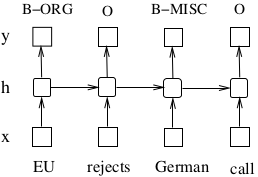
\includegraphics{text/images/rnn.png}
    \caption{RNN~\cite{BiLSTMCRF}}\label{img:rnn}
\end{figure}

\subsection{Long short-term memory network (LSTM)}
Long short-term memory network represents an upgrade of the RNN network that uses a purpose-built memory cell that contains various gates. The memory cell is represented by an input gate $i$, a forget gate $f$, an output gate $o$, and a cell $c$. Due to this approach, LSTM might be more successful than RNN in identifying long-range dependencies in data.

In time $t$ the following equations are computed:
\begin{gather}
    i_t = \sigma(\mathbf{W}_{xi}x_t + \mathbf{W}_{hi}h_{t-1} + \mathbf{W}_{ci}c_{t-1} + b_i)\\
    f_t = \sigma(\mathbf{W}_{xf}x_t + \mathbf{W}_{hf}h_{t-1} + \mathbf{W}_{cf}c_{t-1} + b_f)\\
    c_t = f_tc_{t-1} + i_t\tanh(\mathbf{W}_{xc}x_t + \mathbf{W}_{hc}h_{t-1} + b_c)\\
    o_t = \sigma(\mathbf{W}_{xo}x_t + \mathbf{W}_{ho}h_{t-1} + \mathbf{W}_{co}c_t + b_o)\\
    h_t = o_t\tanh(c_t).
\end{gather}

In the equations, $h$ denotes the hidden vector, $\mathbf{W}$ the weight matrices computed during training, $\sigma$ the sigmoid activation function, and $b$ the bias. The weight matrices from the cell to the gates (e.g.~$\mathbf{W}_{cf}$) are diagonal, and because of this, every element in each gate vector is updated only with the value of the corresponding element in the cell vector.~\cite{BiLSTMCRF}

For an LSTM memory cell schema, see Figure~\ref{img:lstm-cell}. For a network schema, see Figure~\ref{img:lstm}.

\begin{figure}[htbp]
    \centering
    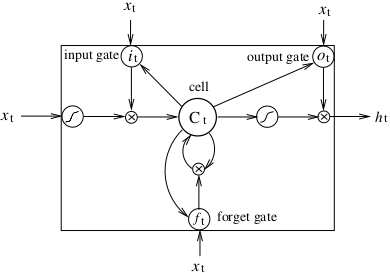
\includegraphics{text/images/lstm_cell.png}
    \caption{LSTM memory cell~\cite{BiLSTMCRF}}\label{img:lstm-cell}
\end{figure}

\begin{figure}[htbp]
    \centering
    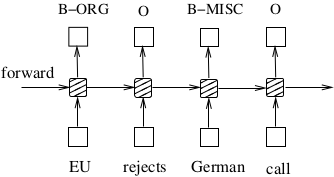
\includegraphics{text/images/lstm.png}
    \caption{LSTM network~\cite{BiLSTMCRF}}\label{img:lstm}
\end{figure}

\subsection{Bidirectional LSTM network (BiLSTM)}
Using RNNs and LSTM networks has one major flaw: for each input, the output is predicted using only the previous input information. Information about future inputs cannot be incorporated. The bidirectional LSTM network solves this problem.

The BiLSTM network contains two LSTM networks: forward, which processes the input sequence from left to right, and backward, which processes it from right to left. The output for a time step is then obtained using information encoded in both networks. The entire network can be trained using the backpropagation through time algorithm.~\cite{BiLSTMCRF} For a network illustration, see Figure~\ref{img:bilstm}.

\begin{figure}[htbp]
    \centering
    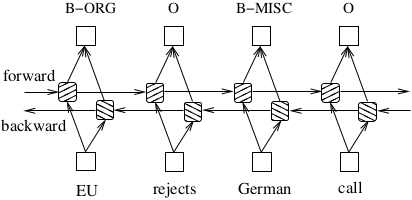
\includegraphics{text/images/bilstm.png}
    \caption{BiLSTM network~\cite{BiLSTMCRF}}\label{img:bilstm}
\end{figure}

\subsection{Conditional random fields network (CRF)}
Unlike the previous approaches, conditional random fields focus on the entire sequence rather than individual positions when finding the optimal tagging. In this model, the inputs and outputs are directly connected. There are no recurrent cells as in the previous approaches (see Figure~\ref{img:crf}).~\cite{BiLSTMCRF} For details, see \cite{CRF}.

\begin{figure}[htbp]
    \centering
    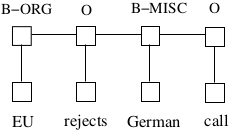
\includegraphics{text/images/crf.png}
    \caption{CRF network~\cite{BiLSTMCRF}}\label{img:crf}
\end{figure}

\subsection{LSTM-CRF network}
LSTM-CRF network combines the LSTM and the CRF network into one model.
When predicting the current tag, it can use information on previous inputs from the LSTM layer, as well as sequence-level information on past and future tags from the CRF layer.~\cite{BiLSTMCRF} For an illustration, see Figure~\ref{img:lstm-crf}.

\begin{figure}[htbp]
    \centering
    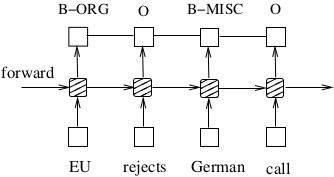
\includegraphics{text/images/lstm_crf.png}
    \caption{LSTM-CRF network~\cite{BiLSTMCRF}}\label{img:lstm-crf}
\end{figure}

\subsection{Bidirectional LSTM-CRF network (Bi\-LSTM-CRF)}
The bidirectional LSTM-CRF network combines the BiLSTM and the CRF network into one model. Unlike the LSTM-CRF network, it uses information about future inputs when predicting the current tag. It represents the current state-of-the-art model for standard sequence tagging tasks such as POS or NER tagging.~\cite{BiLSTMCRF} For an illustration of the network architecture, see Figure~\ref{img:bi-lstm-crf}.

\begin{figure}[htbp]
    \centering
    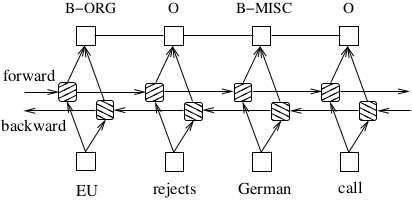
\includegraphics{text/images/bilstm_crf.png}
    \caption{BiLSTM-CRF network~\cite{BiLSTMCRF}}\label{img:bi-lstm-crf}
\end{figure}

\subsubsection{Training procedure}
The BiLSTM-CRF network is trained using the procedure described in Figure~\ref{fig:bi-lstm-crf-trainig}. Multiple training epochs are performed. In each epoch, the training data are divided into equal-sized batches processed independently. First, the BiLSTM network performs forward passes for both its LSTM networks, forward and backward. As a result, the output score $f_{\theta}(w)$ is obtained for all tags at all positions, where $\theta$ represents the parameters of the BiLSTM network and $w$ represents the input sequence. After that, a CRF layer forward and backward passes are run to compute
gradients for the BiLSTM network output and state transition
edges in the CRF layer. The errors are then backpropagated to the input using the backward passes of the BiLSTM network. Finally, all network parameters -- the state transition matrix of the CRF layer and the parameters $\theta$ of the BiLSTM network -- are updated.~\cite{BiLSTMCRF}

\begin{figure}[htbp]
    \centering
  \begin{algorithmic}
    \FOR{each epoch}
        \FOR{each batch}
        \STATE bidirectional LSTM-CRF model forward pass:
            \STATE \quad forward pass for forward state LSTM
            \STATE \quad forward pass for backward state LSTM
        \STATE CRF layer forward and backward pass
        \STATE bidirectional LSTM-CRF model backward pass:
            \STATE \quad backward pass for forward state LSTM
            \STATE \quad backward pass for backward state LSTM
       \STATE update parameters
      \ENDFOR
    \ENDFOR
  \end{algorithmic}
  \caption{BiLSTM-CRF network: Training procedure}\label{fig:bi-lstm-crf-trainig}
\end{figure}

\subsubsection{Input features}
Representation of a word inputted into the BiLSTM-CRF network can consist of multiple concatenated vectors: word embedding, capitalisation feature, and character-based representation.~\cite{BiLSTMCRFHyperparameters} For illustration, see Figure~\ref{img:bi-lstm-crf-input}.

\begin{figure}[htbp]
    \centering
  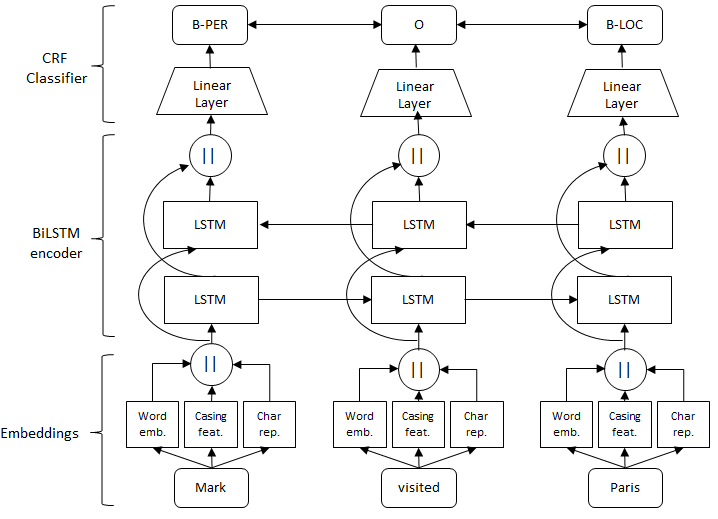
\includegraphics[width=\textwidth]{text/images/bilstm_crf_input.png}
  \caption{BiLSTM-CRF network: Input features~\cite{BiLSTMCRFHyperparameters}}\label{img:bi-lstm-crf-input}
\end{figure}

\paragraph{Word embeddings}
Word embeddings can be used already pre-trained on large text corpora or can be pre-trained on the training data. Popular algorithms for training word embeddings are, for example, GloVe, FastText (which uses n-grams of words)~\cite{BiLSTMCRFHyperparameters}, Word2Vec~\cite{Word2Vec}, or ELMo~\cite{ELMo}.

\paragraph{Capitalisation feature}
Since pre-trained word embeddings usually exist only for lowercase words, a one-hot vector representing the original capitalisation tends to be used. It can preserve information about whether the inputted word is entirely or mainly numeric, has all characters upper or lowercase, starts with an uppercase character, or contains some digit.~\cite{BiLSTMCRFHyperparameters}

\paragraph{Character-based representation}
Information about the characters of a word can also be added to the input. Two different methods can be used: to derive embedding representing characters of a word using BiLSTM or use convolutional neural networks (CNN).~\cite{BiLSTMCRFHyperparameters}

\subsubsection{Training hyperparameters}
When training the BiLSTM-CRF, various hyperparameters of the network can be fine-tuned.

\paragraph{Optimizer}
While training the network, an objective function is minimised using some optimizer. A commonly used optimizer represents stochastic gradient descent (SGD). However, SGD can be quite sensitive to selecting the learning rate and can have trouble navigating ravines and saddle points. Therefore, other gradient-based optimization algorithms have been proposed, such as Adagrad, Adadelta, RMSProp, Adam, or Nadam (Adam variant that incorporates Nesterov momentum).~\cite{BiLSTMCRFHyperparameters}

\paragraph{Dropout}
Dropout is a method that helps prevent overfitting when training a neural network. 

\subparagraph{Naive dropout}
The naive dropout strategy applies a randomly selected dropout mask to each LSTM output. Different masks are generated for each time step, and recurrent connections are not dropped. It was noted that this form of dropout is suboptimal for recurrent neural networks.

\subparagraph{Variational dropout}
The optimal dropout for recurrent neural networks represents the variational dropout. It uses the same dropout mask for all time steps. Moreover, it drops the recurrent connections as well.~\cite{BiLSTMCRFHyperparameters}

\paragraph{Gradient clipping and normalization}
When a recurrent neural network is trained, two common issues can be encountered: \emph{vanishing gradient} and \emph{exploding gradient} problem. The vanishing gradient problem is countered by using LSTM networks instead of RNNs. To deal with the exploding gradient problem, two common strategies can be applied: gradient clipping and gradient normalization.

\subparagraph{Gradient clipping}
Gradient clipping clips the gradient's components element-wise so that they do not exceed a defined threshold.

\subparagraph{Gradient normalization}
Gradient normalization has a better theoretical justification than gradient clipping. It rescales the gradient whenever the norm of the gradient goes over a defined threshold.~\cite{BiLSTMCRFHyperparameters}

\chapter{Metrical analysis of Czech syllabotonic verse}\label{chap:metrical-analysis}

\begin{chapterabstract}
This chapter describes the pipeline to follow when performing the metrical analysis of Czech syllabotonic verse. It presents all subtasks along with possible approaches to solve them.
\end{chapterabstract}

%---------------------------------------------------------------
\section{Syllabification}
%---------------------------------------------------------------
When performing a metrical analysis of verse, the first step is to split the text into syllables. Perform the so-called syllabification.

\subsection{Syllable in Czech}
For a native speaker, the question of how many syllables are there in a word is generally relatively easy to answer. Why? Inside every syllable, there is a sonority peak. In Czech, the sonority peak can be expressed by:

\begin{enumerate}
    \item Vocal or diphthong.
    \item Sonorant \emph{r} or \emph{l} when positioned between two consonants or at the end of a word after at least one consonant, e.g.~\emph{krk}, \emph{vlk}.
    \item In some exceptional cases also nasals or sibilants, e.g.~\emph{osm}, \emph{pst}, \emph{sedm}.
\end{enumerate}

Words without the sonority peak -- non-syllabic prepositions \emph{v}, \emph{k}, \emph{s}, and \emph{z} -- form one syllable with the first syllable of the following word.

On the other hand, determining syllable boundaries is a challenge even for a native speaker. For example, the Czech word \emph{houska}. It obviously consists of two syllables, but how to split it? \emph{Hou-ska} or \emph{hous-ka}? There is no correct answer.~\cite{UvodTeorieVerse}

\subsection{Syllabification using phonetic transcription}
So, native speakers can easily determine the number of syllables in a word, but how to do it using a computer? The KVĚTA~\cite{KVETA} program applies a sequence of rules to the input words and obtains their phonetic transcriptions. This is possible because the Czech orthography is highly phonemic. The only words that cannot be transcribed using a set of rules are words containing bigrams and foreign words.

As there seems to be no efficient algorithm to automatically decide which instances of the bigrams \emph{au}, \emph{ou} and \emph{eu} represent a diphthong (e.g.~\emph{koule}) and which represent two standalone vowels (e.g.~\emph{pouliční}), KVĚTA transcribes them using a manually built token-diphthong library and applying a few additional rules. Another problem is irregularities when, for example, words like \emph{nauka} or \emph{Zeus} are treated in some poems as disyllabic and in other poems as monosyllabic. Such irregularities are revealed when KVĚTA tries to assign the most probable metre to a poem. The correct variant must then be selected manually.

When dealing with words from other languages, a possible approach would be to identify the most probable donor language and apply the transcription rules of this language. However, since there are many counterexamples as to why this approach would not be efficient, KVĚTA authors decided to also transcribe foreign words using a manually built library. For some words where the number of syllables differs depending on the case (e.g.~\emph{Shakespeare}) or depending on the pronunciation (e.g.~\emph{Baudelaire}) the selection of the right variant is also done manually.~\cite{KVETA}

\subsection{Syllabification using hyphenation tools}
Thus, for each word, the number of syllables can be obtained from its phonetic transcription. However, is there no way to obtain the number of syllables in a word without having its phonetic transcription? And to also extract the individual syllables?~\cite{GitCorpusCzechVerse}

There exist some tools for the hyphenation of Czech texts. Hyphenation seems like a task similar to syllabification but, in fact, it is something a little different. Hyphenation is nowadays used within every document preparation system (e.g.~\TeX{} or any modern web browser) to decide where a word can be split to continue on the following line. There are two approaches to hyphenation:

\begin{itemize}
    \item etymology-based,
    \item phonology-based.
\end{itemize}

Etymology-based systems cut words on the border of a compound word or the border of the stem and ending or prefix or negation. Phonology-based systems cut words based on the pronunciation of syllables.~\cite{TowardsUniversalHypenation} However, they do not cut words directly into individual syllables. Other typographical rules are applied, such as that the first and the last letter of a word cannot be hyphenated (e.g.~the word \emph{italština} is hyphenated as \emph{ital-šti-na}) or that words containing less than five letters are not hyphenated.~\cite{HyphenateBatchelder}

The approach of using hyphenation tools for syllabification has already been tested by researchers when performing metrical analysis of English and German verse using machine learning. For English verse they decided to train BiLSTM-CRF syllabification model instead, for German verse they used an ensemble of hyphenation tools and heuristic corrections.~\cite{MetricalTaggingInTheWild}

\pagebreak

\section{Detecting accented syllables}
\subsection{Accent in Czech}
When talking about accent in Czech, usually, each initial syllable of a polysyllabic word is considered accented, while each non-initial non-accented. For monosyllabic words, the rules are not as clear. The general tendency is that the content words (nouns, adjectives, numerals, interjections, and verbs, except for forms of the lemma \emph{být}) are accented, while the function words are non-accented.

A special case is monosyllabic prepositions proper (MPPs), which usually behave as forming a~single word with the following one and taking over its accent. However, sometimes MPPs can also be used as standard non-accented function words. This has been largely exploited by poets, especially in the second half of the 19\textsuperscript{th} century.~\cite{KVETA} Also the longer the subsequent word, the greater the tendency to have an accent not only on the MPP but also on the subsequent word, e.g.~\emph{\uline{na} \uline{me}zinárodní \uline{le}tiště}.~\cite{UvodTeorieVerse} MPPs are represented by these prepositions: \emph{před}, \emph{od}, \emph{ob}, \emph{ku}, \emph{ke}, \emph{do}, \emph{ve}, \emph{po}, \emph{nad}, \emph{přes}, \emph{při}, \emph{bez}, \emph{se}, \emph{ze}, \emph{za}, \emph{u}, \emph{pod}, \emph{pr}o and \emph{zpod}. In the case of two subsequent MPPs, the first is considered a standard function word.~\cite{KVETA}

\section{Metre assignment}
In this section, two approaches to the metrical tagging of Czech syllabotonic verse are presented: a rule-based approach that the KVĚTA program used in the past~\cite{TowardsAutomaticAnalysis} and a data-driven approach that the current version of the KVĚTA program is using.~\cite{KVETA}

\subsection{Rule-based KVĚTA algorithm}
All the following information is taken from~\cite{TowardsAutomaticAnalysis}.

\subsubsection{Prosodic analysis}
The first step of the rule-based algorithm is to represent a line of verse as a string containing symbols \emph{0}, \emph{1} and \emph{+}, where \emph{1} represents an accented syllable, \emph{0} a non-accented syllable, and a \emph{+} a monosyllable. Monosyllables can be both accented and non-accented. In the case of a~monosyllabic preposition, the preposition itself is treated as an initial syllable of a polysyllabic unit and the following syllable as a non-initial syllable of a polysyllabic unit. For the transcription rules, see Table~\ref{tab:kveta-rule-based-transcription-rules}.

\begin{table}[htpb]
\centering
\caption{Rule-based KVĚTA algorithm: Prosodic transcription rules}\label{tab:kveta-rule-based-transcription-rules}
\begin{tabular}{|c||l|}\hline
    Syllable type & Symbol\\\hline\hline
    First syllable of a polysyllabic unit & 1\\
    Non-initial syllable of a polysyllabic unit & 0\\
    Monosyllable & +\\\hline
\end{tabular}
\end{table}

The sentence \enquote{Za trochu lásky šel bych světa kraj} is represented by a primary string:
\begin{verbatim}
10010++10+.
\end{verbatim}

The problem is that poets do not produce purely metrical lines. Therefore, in addition to the primary string, the algorithm also analyses three alternative strings applying the three most common stress alterations:
\begin{enumerate}
    \item Treating the sequence of a monosyllabic preposition and another unit as having the stress located not on the first syllable (preposition) but on the second one (\verb|100 -> +10|).
    \item Relocating the stress of a polysyllabic unit (incidental prepositions included) to the immediately preceding monosyllable (\verb|+10 -> 100|).
    \item Tolerating that stress of one polysyllabic unit occupies one of the forbidden positions.
\end{enumerate}

\subsubsection{Metrical analysis}
The metrical analysis is based on the following simplified rules of Czech syllabotonic verse:

\begin{enumerate}
    \item A line is iambic (I) if no odd position except the first (allowing dactylic incipits) is occupied by the stress of a polysyllabic unit.
    \item A line is trochaic (T) if no even position is occupied by the stress of a polysyllabic unit.
    \item \label{item:kveta-rule-based-rules-3} A line is dactylic (D) if for each $n = 0, 1, 2, \ldots$
        \begin{enumerate}
            \item no (3n+3)\textsuperscript{rd} position is occupied by the stress of a polysyllabic unit and
            \item \label{item:kveta-rule-based-rules-3b} no (3n+2)\textsuperscript{nd} position is occupied by the stress of a unit consisting of three or more syllables and
            \item \label{item:kveta-rule-based-rules-3c} every stress occupying a (3n+2)\textsuperscript{nd} position is preceded by a monosyllabic unit.
        \end{enumerate}
    \item \label{item:kveta-rule-based-rules-4} A line is dactylic with anacrusis (Da) if for each $n = 0, 1, 2, \ldots$
        \begin{enumerate}
            \item the first position is occupied by a monosyllabic unit and
            \item \label{item:kveta-rule-based-rules-4b} no (3n+4)\textsuperscript{th} position is occupied by the stress of a polysyllabic unit and
            \item \label{item:kveta-rule-based-rules-4c} no (3n+3)\textsuperscript{rd} position is occupied by the stress of a unit consisting of three or more syllables and
            \item every stress occupying a (3n+3)\textsuperscript{rd} position is preceded by a monosyllabic unit.
        \end{enumerate}
    \item A line is dactylo-trochaic (DT) if a \enquote{virtual syllable} can be inserted into the line after some of the 3n+2 nd positions (at least once) in order to meet the conditions specified in~\ref{item:kveta-rule-based-rules-3}.
    \item A line is dactylo-trochaic with anacrusis (DTa) if the \enquote{virtual syllable} can be inserted into the line after some of the 3n+3\textsuperscript{rd} positions (at least once) in order to meet the conditions specified in~\ref{item:kveta-rule-based-rules-4}.
\end{enumerate}

The metrical tagging procedure is visualised on a sample from Karel Hynek Mácha's \emph{Máj} -- an iambic poem, yet with iambic constraints frequently violated in various ways. Row 0 shows the primary string, and rows I-III show the alternative strings that allow for stress alterations. Positions within the string that violate the constraints of a given metre are highlighted. The first string in a column that does not violate the constraints of a given metre or violates it only once (row III) is underlined:

\pagebreak

Zhasla měsíce světlá moc,\\
\begin{center}
\begin{tabular}{c||m{2.5cm}|m{2.5cm}|m{2.5cm}|m{3.5cm}}
    Row & Iamb & Trochee & Dactyl & Dactyl with anacrusis\\\hline\hline
    0 & 10\textbf{1}0010+ & 10100\textbf{1}0+ & 10\textbf{1}00\textbf{1}0+ & \textbf{1}0\textbf{1}00\textbf{1}0+\\
    I & 10\textbf{1}0010+ & 10100\textbf{1}0+ & 10\textbf{1}00\textbf{1}0+ & \textbf{1}0\textbf{1}00\textbf{1}0+\\
    II & 10\textbf{1}0010+ & 10100\textbf{1}0+ & 10\textbf{1}00\textbf{1}0+ & \textbf{1}0\textbf{1}00\textbf{1}0+\\
    III & \underline{10\textbf{1}0010+} & \underline{10100\textbf{1}0+} & 10\textbf{1}00\textbf{1}0+ & \textbf{1}0\textbf{1}00\textbf{1}0+\\
\end{tabular}
\end{center}

Output: Iamb / Trochee

i hvězdný svit a kol a kol\\
\begin{center}
\begin{tabular}{c||m{2.5cm}|m{2.5cm}|m{2.5cm}|m{3.5cm}}
    Row & Iamb & Trochee & Dactyl & Dactyl with anacrusis\\\hline\hline
    0 & \underline{+10+++++} & +\textbf{1}0+++++ & \underline{+10+++++} & \underline{+10+++++}\\
    I & +10+++++ & +\textbf{1}0+++++ & +10+++++ & +10+++++\\
    II & 100+++++ & \underline{100+++++} & 100+++++ & \textbf{1}00+++++\\
    III & +10+++++ & +\textbf{1}0+++++ & +10+++++ & +10+++++\\
\end{tabular}
\end{center}

Output: Iamb / Trochee / Dactyl / Dactyl with anacrusis

\begin{center}
je pouhé temno, širý dol\\
\begin{tabular}{c||m{2.5cm}|m{2.5cm}|m{2.5cm}|m{3.5cm}}
    Row & Iamb & Trochee & Dactyl & Dactyl with anacrusis\\\hline\hline
    0 & \underline{+101010+} & +\textbf{1}0\textbf{1}0\textbf{1}0+ & +1010\textbf{1}0+ & +10\textbf{1}0\textbf{1}0+\\
    I & +101010+ & +\textbf{1}0\textbf{1}0\textbf{1}0+ & +1010\textbf{1}0+ & +10\textbf{1}0\textbf{1}0+\\
    II & 1001010+ & 100\textbf{1}0\textbf{1}0+ & 10010\textbf{1}0+ & \textbf{1}00\textbf{1}0\textbf{1}0+\\
    III & +101010+ & +\textbf{1}0\textbf{1}0\textbf{1}0+ & \underline{+1010\textbf{1}0+} & +10\textbf{1}0\textbf{1}0+\\
\end{tabular}
\end{center}

Output: Iamb / Dactyl

co hrob daleký zívá.\\
\begin{center}
\begin{tabular}{c||m{2.5cm}|m{2.5cm}|m{2.5cm}|m{3.5cm}}
    Row & Iamb & Trochee & Dactyl & Dactyl with anacrusis\\\hline\hline
    0 & ++\textbf{1}0010 & ++100\textbf{1}0 & ++\textbf{1}00\textbf{1}0 & ++\textbf{1}00\textbf{1}0\\
    I & ++\textbf{1}0010 & ++100\textbf{1}0 & ++\textbf{1}00\textbf{1}0 & ++\textbf{1}00\textbf{1}0\\
    II & \underline{+100010} & +\textbf{1}000\textbf{1}0 & +\textbf{1}000\textbf{1}0 & +1000\textbf{1}0\\
    III & ++\textbf{1}0010 & \underline{++100\textbf{1}0} & ++\textbf{1}00\textbf{1}0 & ++\textbf{1}00\textbf{1}0\\
\end{tabular}
\end{center}

Output: Iamb / Trochee

The final metre for the poem is selected based on a \enquote{metrical index} value. The metrical index of a line is computed as follows:
\begin{itemize}
    \item If at any step a line is assigned a metre, the metrical index of that metre has the value of 100.
    \item Every stress of a disyllabic unit according to rules~\ref{item:kveta-rule-based-rules-3b}/\ref{item:kveta-rule-based-rules-3c} or~\ref{item:kveta-rule-based-rules-4b}/\ref{item:kveta-rule-based-rules-4c} except for
the second position (allowing iambic incipits in the dactylic verse) lowers the metrical index value by 20.
    \item If the metre is assigned at row I, metrical index is lowered by 40.
    \item If the metre is assigned at row II, metrical index is lowered by 60.
    \item If the metre is assigned at row III, metrical index is lowered by 80.
    \item Negative values are set to 0.
 \end{itemize}

For every metre, the arithmetic mean of the line metrical indices is computed. The metre with the highest mean value, that further meets the condition of having the mean value higher than 50 and containing no line with a metrical index of 0, is finally selected. For the Mácha's \emph{Máj} example, Iamb is selected:

\begin{center}
\begin{tabular}{c||l|l|l|l}
    & Iamb & Trochee & Dactyl & Dactyl with anacrusis\\\hline\hline
    Zhasla měsíce světlá moc, & 20 & 20 & 0 & 0\\
    i hvězdný svit a kol a kol & 100 & 40 & 100 & 100\\
    je pouhé temno, širý dol & 100 & 0 & 20 & 0\\
    co hrob daleký zívá. & 40 & 20 & 0 & 0\\\hline\hline
    Arithmetic mean & \underline{65} & 20 & 30 & 25\\
\end{tabular}
\end{center}

\subsubsection{Multimetric lines}
In this approach, the metre for a multimetric line is selected depending on the context: the metres of other lines. For multimetric poems that can be assigned multiple metres to an equal degree, preference rules are applied.

\subsubsection{Conclusion}
To conclude, this algorithm can be used for the metrical tagging of Czech syllabotonic verse. Because of the inability of the algorithm to decide whether a monosyllable is accented or not, distinctions among some rare types of dactylo-trochee may not be recognised. Polymetric poem tagging is also not possible. Furthermore, this algorithm does not tag hexametre and pentametre poems, which are tagged within the Corpus of Czech Verse.

\subsection{Data-driven KVĚTA algorithm}
All the following information comes from~\cite{KVETA}.

\subsubsection{Syllable classes}
\begin{table}[hptb]
\centering
\caption{Data-driven KVĚTA algorithm: Syllable class structure}\label{tab:kveta-data-driven-syllable-class-structure}
\begin{tabular}{|c||l|}\hline
    Parameter & Values\\\hline\hline
    initial & \begin{tabular}{@{}l@{}}1 (word-initial syllable)\\0 (non-initial syllable)\end{tabular}\\\hline
    final & \begin{tabular}{@{}l@{}}1 (word-final syllable)\\0 (non-final syllable)\end{tabular}\\\hline
    contentWord & \begin{tabular}{@{}l@{}}1 (content-word)\\0 (function word)\end{tabular}\\\hline
    preposition & \begin{tabular}{@{}l@{}}1 (MPP preposition)\\0 (other word)\end{tabular}\\\hline
    prevPreposition & \begin{tabular}{@{}l@{}}1 (preceded by MPP preposition)\\0 (preceded by other word)\end{tabular}\\\hline
    prevInitial & \begin{tabular}{@{}l@{}}1 (preceded by word-initial syllable)\\0 (preceded by non-initial syllable)\end{tabular}\\\hline
    nextlong & \begin{tabular}{@{}l@{}}1 (followed by syllable containing long vowel or diphtong)\\0 (followed by other syllable)\end{tabular}\\\hline
\end{tabular}
\end{table}

The data-driven KVĚTA approach represents every syllable as a so-called Syllable class. The Syllable class is a data class containing Boolean parameters (see Table~\ref{tab:kveta-data-driven-syllable-class-structure}) extracted from the Czech accent rules. A poem is then internally represented as a list of lists of Syllable classes, the division into stanzas is not taken into account.

In theory, there are 128 different combinations of parameter values, but in practise many of those are discarded as, e.g.~\verb|{initial: 0, preposition: 1}| or \verb|{final: 0, preposition: 1}|. Another example is the contentWord parameter, which is used only for monosyllabic words that are not preceded by MPP preposition \verb|{initial: 1, final: 1, prevPreposition: 0}|. In addition, the parameters nextLong and prevInitial are taken into account only for a word-initial syllable of a polysyllabic word \verb|{initial: 1, final: 0}| or MPP preposition \verb|{preposition: 1}|. More such reductions are applied, resulting in only 12 recognised Syllable class instances.

For example, the Syllable class instance for the third syllable (\emph{Zná}) of a line: \enquote{Aj! kdo zná ji, tu osobu} is:

\begin{verbatim}
{
    initial: 1,
    final: 1,
    contentWord: 1,
    preposition: 0,
    prevPreposition: 0,
    prevInitial: 1,
    nextLong: 0
}.
\end{verbatim}

\subsubsection{Metre generation}
The next step of the algorithm is to take for each poem only the number of syllables in each line and generate all possible metres that could fit it. Not only standard syllabotonic metres are generated, but also syllabotonic imitations of quantitative syllabic strophes and syllabotonic imitations of the quantitative hexametre, pentametre, and elegiac couplet. Ghazal poems are generated as well. The V-positions are not distinguished and are represented as W-positions.

\paragraph{Standard syllabotonic metres}
The maximal number of syllables in one line \verb|max_syll| must be determined when generating all standard syllabotonic metres for a poem. All possible metres are then generated as strings of length \verb|max_syll| that match the regular expression~\eqref{eq:syllabotonic-regex}.

This regular expression represents all valid combinations of Czech syllabotonic feet. For example, if \verb|max_syll| for a poem is equal to 6, the following metres are generated:

\begin{verbatim}
[‘SWSWSW’, ‘SWWSWS’, ‘SWSWWS’, ‘SWWSWW’, ‘WSWSWS’, ‘WSWSWW’, ‘WSWWSW’].
\end{verbatim}

For every metre generated, a two-dimensional array of metrical positions is created, where the metrical pattern of each line is a prefix of the generated metre. For metre \verb|'SWWSWS'| and a poem consisting of a 5-syllable line, a 6-syllable line, and a 3-syllable line, the following array is generated:

\pagebreak

\begin{verbatim}
metre['SWWSWS'] = [
    ['S', 'W', 'W', 'S', 'W'],
    ['S', 'W', 'W', 'S', 'W', 'S'],
    ['S', 'W', 'W']
].
\end{verbatim}

\paragraph{Imitations of quantitative syllabic strophes}
The algorithm supports the four most commonly imitated quantitative syllabic strophes: the Sapphic Stanza, the Third Asclepiad Stanza and two types of the Alcaic Strophe. When the poem meets the syllabic requirements and can be divided into one of these strophes, the algorithm includes this option in the generated metres. For the metrical patterns of the strophes, see Figure~\ref{fig:kveta-data-driven-strophes}.

\begin{figure}[htpb]
\centering
\begin{verbatim}
metre['sapphic'] = [
    ['S', 'W', 'S', 'W', 'S', 'W', 'W', 'S', 'W', 'S', 'W'],
    ['S', 'W', 'S', 'W', 'S', 'W', 'W', 'S', 'W', 'S', 'W'],
    ['S', 'W', 'S', 'W', 'S', 'W', 'W', 'S', 'W', 'S', 'W'],
    ['S', 'W', 'W', 'S', 'W']
]

metre['asclepiad'] = [
    ['S', 'W', 'S', 'W', 'W', 'S', 'W', 'S', 'W', 'W', 'S', 'W', 'W'],
    ['S', 'W', 'S', 'W', 'W', 'S', 'W', 'S', 'W', 'W', 'S', 'W', 'W'],
    ['S', 'W', 'S', 'W', 'W', 'S', 'W'],
    ['S', 'W', 'S', 'W', 'W', 'S', 'W', 'W']
]

metre['alcaicA'] = [
    ['W', 'S', 'W', 'S', 'W', 'S', 'W', 'W', 'S', 'W', 'W'],
    ['W', 'S', 'W', 'S', 'W', 'S', 'W', 'W', 'S', 'W', 'W'],
    ['W', 'S', 'W', 'S', 'W', 'S', 'W', 'S', 'W'],
    ['S', 'W', 'W', 'S', 'W', 'W', 'S', 'W', 'S', 'W']
]

metre['alcaicB'] = [
    ['S', 'W', 'S', 'W', 'W', 'S', 'W', 'W', 'S', 'W', 'W'],
    ['S', 'W', 'S', 'W', 'W', 'S', 'W', 'W', 'S', 'W', 'W'],
    ['S', 'W', 'S', 'W', 'S', 'W', 'S', 'W', 'W'],
    ['S', 'W', 'W', 'S', 'W', 'W', 'S', 'W', 'S', 'W']
]
\end{verbatim}
\caption{Syllabotonic imitations of quantitative syllabic strophes: Metrical patterns}\label{fig:kveta-data-driven-strophes}
\end{figure}

\paragraph{Imitations of hexametre, pentametre and elegiac couplet}
For a poem that imitates the quantitative hexametre, every line must match the hexametre regular expression~\eqref{eq:hexametre-regex}. That implies that the length of every line varies from 12 to 17 syllables. Moreover, when the length of the line lies between 13 and 16 syllables, there is more than one possible metrical pattern. There are five different patterns for lines of lengths 13 and 16 and ten patterns for lines of lengths 14 and 15. Therefore, a three-dimensional array instead of a~two-dimensional array must be generated. For a poem consisting of a 13-syllable line and a 12-syllable line, the following array is generated:

% \pagebreak

\begin{verbatim}
metre['hexametre'] = [
    [
        ['S', 'W', 'W', 'S', 'W', 'S', 'W', 'S', 'W', 'S', 'W', 'S', 'W'],
        ['S', 'W', 'S', 'W', 'W', 'S', 'W', 'S', 'W', 'S', 'W', 'S', 'W'],
        ['S', 'W', 'S', 'W', 'S', 'W', 'W', 'S', 'W', 'S', 'W', 'S', 'W'],
        ['S', 'W', 'S', 'W', 'S', 'W', 'S', 'W', 'W', 'S', 'W', 'S', 'W'],
        ['S', 'W', 'S', 'W', 'S', 'W', 'S', 'W', 'S', 'W', 'W', 'S', 'W']
    ],
    [
        ['S', 'W', 'S', 'W', 'S', 'W', 'S', 'W', 'S', 'W', 'S', 'W']
    ]
].
\end{verbatim}

For imitation of the quantitative pentametre, the situation is analogous. This time, all lines must match the pentametre regular expression~\eqref{eq:pentametre-regex}. Line lengths range from 10 to 15 syllables, again resulting in a three-dimensional array.

In imitation of the elegiac couplet, all odd lines must match the hexametre regular expression, and all even lines must match the pentametre regular expression. Again, a three-dimensional array is returned.

\paragraph{Ghazal poems}
When a poem is identified as a ghazal poem, the algorithm splits the poem into two separate parts -- part without the radifs and a part containing only the radifs. Possible metrical patterns are generated for each part separately, and the final metrical patterns are returned as their Cartesian product.

\subsubsection{Metre assignment}
\paragraph{Metrical coefficient}
To be able to assign metres, the algorithm must pre-calculate the values of \enquote{metrical coefficient} from the corpus data. For every Syllable class, the metrical coefficient value is represented as the conditional probability that the Syllable class is realised by a strong or weak position in the corresponding metrical pattern. For the $j^{th}$ syllable of the $i^{th}$ line of a poem, and a metre $w$ (which was generated for this poem as a possible metre in the previous step of the algorithm) let $\mu_{w,i,j}$ be the value of the metrical coefficient for that syllable and metre $w$, $\sigma_{i,j}$ the Syllable class assigned to that syllable and $x_{w,i,j}$ the strong or weak position in the metrical pattern of metre $w$.

The authors of the paper use Bayes' Theorem (under a naive independence assumption):

\begin{equation}
    \mu_{w,i,j} = P(x_{w,i,j}|\sigma_{i,j}) = \frac{P(\sigma_{i,j}|x_{w,i,j})\cdot P(x_{w,i,j})}{P(\sigma_{i,j}|S) + P(\sigma_{i,j}|W)}
\end{equation}

and argue that since $x_{w,i,j}$ is a binary value with possible values S or W, the probability of which may be considered equal, they can internally compute $\mu_{w,i,j}$ just as:
\begin{equation}\label{eq:kveta-data-driven-0}
    \tilde{\mu}_{w,i,j} = \frac{P(\sigma_{i,j}|x_{w,i,j})}{P(\sigma_{i,j}|S) + P(\sigma_{i,j}|W)}.
\end{equation}

Moreover, the algorithm also takes into account that the probabilities can vary greatly depending on the time period or individual authors. Therefore, for each author, the Yates $\chi^2$ test is performed to determine whether the probabilities obtained from his work differ statistically significantly from the probabilities of the entire corpus. If they do, his values of the metrical index are set as a geometric mean of the probabilities from the whole corpus and of his probabilities ($P_A$) with a weight ratio of 1 to 3:

\begin{equation}\label{eq:kveta-data-driven-1}
    \mu_{w,i,j} = \sqrt[4]{P(x_{w,i,j}|\sigma_{i,j})\cdot(P_A(x_{w,i,j}|\sigma_{i,j}))^3}.
\end{equation}

\paragraph{Metre selection}
When selecting a metre, the metrical coefficients of the individual line patterns and the overall metrical coefficient must be determined for every generated metre.

For the $i^{th}$ line of a poem and a metre $w$, the metrical coefficient of the line pattern $L_{w,i}$ represents the probability of this line being realised by the metre $w$. It is computed as a product of metrical coefficients of all individual syllables on the line, and it is normalised by the length of the line denoted as $n_i$, so lines of different lengths are comparable:

\begin{equation}\label{eq:kveta-data-driven-2}
    L_{w,i} = \sqrt[n_i]{\prod_{j=1}^{n_i}\tilde{\mu}_{w,i,j}}.
\end{equation}

In the case of the three-dimensional hexametre, pentametre, or elegiac couplet arrays, the line pattern with the highest value of $L_{w,i}$ is selected (out of $k$ possible patterns):

\begin{equation}\label{eq:kveta-data-driven-3}
    L_{w,i} = \max\{L_{w,i,1}, L_{w,i,2}, \ldots, L_{w,i,k}\}.
\end{equation}

The overall metrical coefficient $T_w$ of the metre $w$ is calculated as a geometric mean of the metrical coefficients of all line patterns:

\begin{equation}\label{eq:kveta-data-driven-4}
    T_w = \sqrt[m]{\prod_{i=1}^{m}L_{w,i}},
\end{equation}

where $m$ is the number of lines.

Finally, the metre $w$ with the highest metrical coefficient $T_w$ is selected. Inside KVĚTA, various checks must be passed to annotate the poem automatically. For example, if the value of $T_w$ or some $L_{w,i}$ is too low, or the standard deviation of $L_{w,1}, L_{w,2}, \ldots$ is too high, manual control is required. This approach minimises the incorrect annotations of polymetric or non-syllabotonic poems and reveals possible mistakes in phonetic transcriptions. When the same metrical pattern is generated with different metre names (e.g.~hexametre and trochee), standard syllabotonic metres are preferred.

\subsubsection{Conclusion}
In conclusion, this algorithm seems to be more suitable for metrical tagging of Czech syllabotonic verse than the rule-based one. It can distinguish whether a monosyllable is accented or not, it allows for more advanced rules as e.g.~the MPPs are also taken into account, and it also tags hexametres and pentametres, which are tagged within the Corpus of Czech Verse. Again, polymetric tagging of poems is not possible.

\section{Machine learning approaches}\label{section:ml-approaches}
The metrical analysis can be modelled as a sequence tagging task and solved using machine learning. In the paper~\cite{MetricalTaggingInTheWild}, conditional random fields, BERT model and BiLSTM-CRF model are tested on English and German verse corpora. The paper~\cite{ComparisonFeatureBasedNeualScansion} tests perceptron, hidden Markov model (HMM), conditional random fields, and BiLSTM-CRF on English and Spanish verse corpora. Both articles evaluate syllable-level and line-level accuracies and obtain the best results using BiLSTM-CRF.

\subsection{BERT}
The authors of~\cite{MetricalTaggingInTheWild} assume that BERT's transformer architecture cannot compete against other models, possibly because of an improper syllable representation, as BERT's word-piece tokenizer creates word chunks that are not equivalent to syllables.

Another experiment is performed in which BERT should learn the verse label (e.g.~iambic pentameter) for a given sequence of word tokens. BERT detects frequent classes like the iambic pentameter or the trochaic tetrameter well but fails to learn measures other than iamb, trochee and irregular verse with inversions. The authors assume that BERT probably mainly predicts based on the length of lines in this setting.

\subsection{BiLSTM-CRF}
In~\cite{MetricalTaggingInTheWild}, individual syllables are sent to the input and custom syllable embeddings are pre-trained from verse corpora using the Word2Vec algorithm. BiLSTM-CRF uses three BiLSTM layers with 100 recurrent units in each layer and uses a linear-chain CRF classifier. Variational dropout is used, with 25~\% dropped in output and recurrent connections. No character-based representation of syllables is used, as it, according to the authors, hurts both speed and accuracy.

Unlike the intuition denoted in~\cite{MetricalTaggingInTheWild}, in~\cite{ComparisonFeatureBasedNeualScansion}, BiLSTM-CRF is used with BiLSTM character-based representation of input tokens. Three different input types are tested: individual syllables, word tokens, and individual syllables with word boundaries. For English, the best results are obtained for individual syllables with word boundaries in the input. For Spanish, the best results are obtained when word tokens are inputted.
\chapter{Implementation}\label{chap:implementation}
\begin{chapterabstract}
This chapter discusses approaches aiming to solve the metrical analysis task. First, the reimplementation of the KVĚTA data-driven approach, later using machine learning and training the BiLSTM-CRF model.
\end{chapterabstract}

\section{Used datasets}\label{section:used-data-sets}
Two different datasets obtained from the Corpus of Czech Verse data are used.

The first dataset contains no polymetric poems, no multimetric verses, no unrecognised metrical positions, and no annotation errors. This dataset contains 57 339 poems.

The second dataset contains no unrecognised metrical positions, no multimetric verses, and no annotations errors as well. However, this time, polymetric poems can be present. This dataset contains 59 661 poems.

Both datasets are divided into training, validation, and testing data using a ratio of 70:15:15. The KVĚTA reimplementation is trained on the training and validation data and tested on the testing data. The BiLSTM-CRF model is trained on the training data, finetuned during training on the validation data, and final results are obtained for the previously unseen testing data.

\section{KVĚTA reimplementation}
\subsection{Syllabification using X-SAMPA transcription}
In the reimplementation of the KVĚTA data-driven approach, a phonetic transcription algorithm is not implemented. Instead, phonetic transcriptions already generated by KVĚTA and published within the Corpus of Czech Verse are used. The X-SAMPA format is parsed to obtain the number of sonority peaks and, therefore, the number of syllables for each word. For the X-SAMPA symbols that are counted, see Tables~\ref{tab:sampa-diphthongs}, \ref{tab:sampa-vocals}, \ref{tab:sampa-long-vocals}, and~\ref{tab:sampa-syllabic-consonant}.

\begin{table}[htpb]
\centering
\caption{X-SAMPA: diphthongs}\label{tab:sampa-diphthongs}
\begin{tabular}{|c||l|l|}\hline
    X-SAMPA Transcription & Example Czech Word & Word Transcription\\\hline\hline
    a\_u & auto (car) & a\_uto / ?a\_uto\\
    E\_u & neuron (neuron) & nE\_uron\\
    o\_u & soud (court) & so\_ut\\\hline
\end{tabular}
\end{table}

\begin{table}[htpb]
\centering
\caption{X-SAMPA: vocals}\label{tab:sampa-vocals}
\begin{tabular}{|c||l|l|}\hline
    X-SAMPA Transcription & Example Czech Word & Word Transcription\\\hline\hline
    a & sad (orchard) & sat\\
    E & pes (dog) & pEs\\
    I & list (leaf) & lIst\\
    o & rok (year) & rok\\
    u & sud (barrel) & sut\\\hline
\end{tabular}
\end{table}

\begin{table}[htpb]
\centering
\caption{X-SAMPA: long vocals}\label{tab:sampa-long-vocals}
\begin{tabular}{|c||l|l|}\hline
    X-SAMPA Transcription & Example Czech Word & Word Transcription\\\hline\hline
    a: & sám (alone) & sa:m\\
    E: & lék (medicine) & lE:k\\
    i: & sýr (cheese) & si:r\\
    o: & tón (tone) & to:n\\
    u: & sůl (salt) & su:l\\\hline
\end{tabular}
\end{table}

\begin{table}[htpb]
\centering
\caption{X-SAMPA: syllabic consonants}\label{tab:sampa-syllabic-consonant}
\begin{tabular}{|c||l|l|}\hline
    X-SAMPA Transcription & Example Czech Word & Word Transcription\\\hline\hline
    = & krk, vlk (throat, wolf) & kr=k, vl=k\\\hline
\end{tabular}
\end{table}

\subsection{Syllable classes}
In the paper~\cite{KVETA} explaining the KVĚTA data-driven approach, the final Syllable class count is reduced to only 12 different Syllable classes. As not all the reductions applied are properly explained in the paper, the reimplementation got to the number of 15 different Syllable classes.

\subsection{Metre generation}
The reimplementation generates the same metres as KVĚTA -- the standard syllabotonic metres; imitations of quantitative syllabic strophes; imitations of hexametre, pentametre, and elegiac couplet; and ghazal poems.

\subsection{Metre assignment}
In the reimplementation, the conditional probability of a Syllable class being realised by a strong or weak position $P(x_{w,i,j}|\sigma_{i,j})$ is not counted using Bayes' Theorem as it is inside KVĚTA (see Equation~\eqref{eq:kveta-data-driven-0}), but is counted directly. In my opinion, counting the probability using Bayes' theorem is, in this case, unnecessary and does not add any benefit compared to counting it directly. Moreover, in my opinion, the probabilities of strong and weak positions should not be considered equal, as the weak position is a bit more likely to occur depending on the structure of all the syllabotonic feet. Probabilities are estimated from training and validation datasets. Yates' $\chi^2$ test is not performed as it adds another complexity to the task, and, therefore, the probabilities are not modified for outlier authors (see Equation~\eqref{eq:kveta-data-driven-1}).

When selecting the metre, the metrical coefficients of the individual line patterns and the overall metrical coefficients are calculated the same as in KVĚTA (see Equations~\eqref{eq:kveta-data-driven-2}, \eqref{eq:kveta-data-driven-3}, and~\eqref{eq:kveta-data-driven-4}). When the same metrical pattern is generated with different metre names, standard syllabotonic metres are selected with priority as in KVĚTA.

\section{BiLSTM-CRF}
Based on the research of machine learning approaches done in Section~\ref{section:ml-approaches}, the BiLSTM-CRF model is selected for training.
 
\subsection{Used implementation}
One of the publicly available implementations of BiLSTM-CRF for sequence tagging~\cite{GitBiLSTMCRF} is used to train the BiLSTM-CRF model. The same implementation is used in the paper~\cite{MetricalTaggingInTheWild}. It uses Keras version 2.2.0 with Tensorflow 1.8.0 as the backend. It must be run using Python 3.6 or lower to be compatible with the Tensorflow version.~\cite{GitBiLSTMCRF}
 
\subsection{Input data format}
When training the BiLSTM-CRF model, two different input data formats are tested:
\begin{itemize}
    \item token-level,
    \item syllable-level.
\end{itemize}

Both formats are inputted using two different approaches:
\begin{itemize}
    \item one input sequence represents a line in a poem,
    \item one input sequence represents a whole poem.
\end{itemize}

For the token-level input data format, the model is inputted a sequence of individual tokens (words) from the poem. For each token, a sequence of metrical positions is predicted. This sequence can be empty as well, when the token is non-accented.

For the syllable-level input data format, the model is inputted a sequence of individual syllables from the poem. For every syllable, exactly one metrical position is predicted. Because the Corpus of Czech Verse lacks annotation of the syllable boundaries, two approaches to obtain syllable-level data are tested: syllabification using hyphenation tools and X-SAMPA syllables.

\subsubsection{Syllabification using hyphenation tools}
Approach to syllabification using phonology-based Czech \TeX{} hyphenation patterns~\cite{UnreasonableEffectiveness} with Frank Liang’s hyphenation algorithm~\cite{HyphenationLiang} is tested. The implementation of Frank Liang’s algorithm published by Ned Batchelder~\cite{HyphenateBatchelder} is modified to support Czech patterns. The problem encountered is that, for example, the word \emph{houska} is hyphenated as \emph{hou-s-ka} due to the ambiguity of the syllable boundaries where both \emph{hous-ka} and \emph{hou-ska} represent valid syllable splits. Therefore, the output has to be further processed to identify and merge these splits.

The next hyphenation tool tested is the Pyphen~\cite{Pyphen} program, which uses Hunspell hyphenation dictionaries and supports the Czech language. It does not annotate both syllable boundaries in case of ambiguity, as Czech \TeX{} hyphenation patterns do.

For the training data of the second dataset used (see Section~\ref{section:used-data-sets}) the average difference from the correct number of syllables in one token is 0.21 for Czech \TeX{} hyphenation patterns, 0.06 for Pyphen and 0.15 for Czech \TeX{} hyphenation patterns with applied heuristics, that one-letter syllables are merged into the previous ones. For Czech \TeX{} hyphenation patterns, on average, 21.63~\% of tokens in one line have an incorrect number of syllables assigned, for Pyphen 6.18~\% and for Czech \TeX{} hyphenation patterns with heuristics 15.31~\%. The referential syllable counts are obtained by splitting X-SAMPA transcriptions using sonority peak symbols (see Tables~\ref{tab:sampa-diphthongs}, \ref{tab:sampa-vocals}, \ref{tab:sampa-long-vocals}, and~\ref{tab:sampa-syllabic-consonant}).

As the differences between the referential syllable counts and the syllable counts obtained by the hyphenation approaches are not so insignificant, it is decided not to use the hyphenation tools at the moment. Furthermore, knowledge about non-syllabic prepositions would have to be incorporated when using these approaches.

\subsubsection{X-SAMPA syllables}
As the hyphenation approaches to syllabification are rejected, X-SAMPA phonetic transcriptions are parsed to obtain syllable representations with correct syllable count. For each word, its X-SAMPA transcription is divided into X-SAMPA syllables using transcriptions of sonority peaks (see Tables~\ref{tab:sampa-diphthongs}, \ref{tab:sampa-vocals}, \ref{tab:sampa-long-vocals}, or and~\ref{tab:sampa-syllabic-consonant}). For non-syllabic words without a sonority peak, no X-SAMPA syllables are generated.

As an example, for the token \emph{blýskajícím} with X-SAMPA transcription \verb|bli:skaji:t_si:m| the following four X-SAMPA syllables are obtained: \verb|[bli:, ska, ji:, t_s:m]|.

\subsection{Input features}
In accordance with the intuition of the paper~\cite{MetricalTaggingInTheWild} no character-based representation of the input is used. The decision is made not to use the capitalisation feature, as the capitalisation of words seems to be of minor importance for this task, and words inside poems usually do not contain numerals.

As word embeddings, Word2Vec embeddings are pre-trained on the training data. By mistake, for the syllable input, Word2Vec embeddings are pre-trained also on the non-syllabic tokens that are not inputted to the model. Due to time reasons, the models are not retrained. However, the assumption is that it should not affect the results significantly.

The implementation supports inputting other features in addition to the input tokens. Following intuition from~\cite{KVETA}, author of a poem, year of publication, POS tag, or lemma is also inputted. An embedding of size 10 is assigned automatically to every input value and concatenated with other input embeddings.

\subsection{Training}
Training loop denoted in Figure~\ref{fig:bi-lstm-crf-trainig} is performed.

The implementation is optimised for speed, it groups sentences with the same lengths together during training, and thanks to that, it is much faster than other BiLSTM-CRF implementations.~\cite{GitBiLSTMCRF} Even though the implementation is highly configurable, the hyperparameters are not further fine-tuned, as training of one input configuration takes 1 to 2 days (CPU is used, training on GPU is not tested).

\subsection{Training hyperparameters}
The hyperparameters are set according to the recommendations in~\cite{MetricalTaggingInTheWild} and~\cite{BiLSTMCRFHyperparameters}.

Following intuition from~\cite{MetricalTaggingInTheWild}, variational dropout is used, which drops 25~\% in the output and recurrent connections, and three BiLSTM layers with 100 recurrent units are trained inside each layer.

In accordance with the findings of~\cite{BiLSTMCRFHyperparameters}, Nadam optimizer is utilised. Thirty-two sentences are used for mini-batch training, as the training set is relatively large. To fight the exploding gradient problem, no gradient clipping, but gradient normalization is performed with threshold value 1. Models are trained for 15 epochs. Training is stopped earlier if the best validation score does not increase for more than five training epochs.

\subsection{Example configuration of hyperparameters}
For a concrete example of the configuration of hyperparameters, see Figure~\ref{fig:bilstm-crf-hyperparameters-config}.

\begin{figure}[htpb]
\centering
\begin{minted}[tabsize=2,breaklines]{js}
{
    "dropout": [0.25, 0.25],
    "classifier": ["CRF"],
    "LSTM-Size": [100, 100, 100],
    "optimizer": "nadam",
    "earlyStopping": 5,
    "miniBatchSize": 32,
    "charEmbeddings": None,
    "clipvalue": 0,
    "clipnorm": 1,
    "featureNames": ["tokens", "lineIdx", "author", "year", "pos", "lemma"],
    "addFeatureDimensions": 10
}
\end{minted}
\caption{BiLSTM-CRF library: Example configuration of hyperparameters}\label{fig:bilstm-crf-hyperparameters-config}
\end{figure}
\chapter{Results}\label{chap:results}

\section{Accuracies}
When testing the metrical analysis approaches implemented, the following accuracies are taken into account:
\begin{description}
    \item[Syllable-level accuracy]: Testing for all individual syllables whether the metrical position assigned to that syllable is the same as the referential.
    \item[Line-level accuracy]: Testing for all individual lines whether the metrical pattern assigned to that line is the same as the referential.
    \item[Poem-level accuracy]: Testing for all individual poems whether the metrical pattern assigned to that poem is the same as the referential.
\end{description}

For BiLSTM-CRF models with token input, syllable accuracies cannot be evaluated because the reference syllable counts and predicted syllable counts tend to differ.

\section{Results}
For the results on both datasets used (see Section~\ref{section:used-data-sets}), see Tables~\ref{tab:results-data-set-0}, \ref{tab:results-data-set-1}.

It can be seen that BiLSTM-CRF represents a great success, as with the best input configurations, it returns better results than the KVĚTA reimplementation, comparing all evaluated accuracies (syllable-level, line-level, and poem-level).

Not surprisingly, the syllable input returns better results than the token input, especially when comparing the poem-level accuracy. However, when only the line-level accuracy is looked at, the results for token input are not that bad. Therefore, these results seem promising; as for token input, prior syllabification is not needed during preprocessing. An interesting observation is that inputting a lemma significantly improves the results for token input. Generally, the more additional features inputted (author of a poem, year of publication, POS tag, lemma), the better the results.

However, the most interesting finding of this work is how much inputting sequences representing whole poems rather than poem lines improves the results (especially the poem-level accuracy and perhaps surprisingly even the syllable-level accuracy). The best results are obtained inputting sequences representing whole poems with all additional features and poem line indices on the input. Poem line indices allow the model to distinguish different lines of a poem.

\begin{table}[htpb]
\centering
\caption[Results for the first dataset]{Results for the first dataset (no polymetric verses, no verse multimetry)}\label{tab:results-data-set-0}
\begin{tabular}{|c||c|c|c|}\hline
    Approach & Syll. acc. & Line acc. & Poem acc.\\\hline\hline
    KVĚTA reimplementation & 97.02 & 81.88 & 69.83\\\hline
    \makecell{BiLSTM-CRF with X-SAMPA syll. embeddings\\Input: X-SAMPA syllables\\Max epochs: 15} & 97.93 & 95.67 & 66.78\\\hline
    \makecell{BiLSTM-CRF with X-SAMPA syll. embeddings\\Input: X-SAMPA syllables, authors, years\\Max epochs: 15} & 98.14 & 95.97 & 66.29\\\hline
    \makecell{BiLSTM-CRF with X-SAMPA syll. embeddings\\Input: X-SAMPA syllables, authors, years, POS tags\\Max epochs: 15} & 98.69 & 96.85 & 72.34\\\hline
    \makecell{BiLSTM-CRF with X-SAMPA syll. embeddings\\Input: X-SAMPA syllables, authors, years, POS tags,\\lemmas\\Max epochs: 15} & 98.74 & 96.94 & 72.98\\\hline
    \makecell{BiLSTM-CRF with X-SAMPA syll. embeddings\\poem as line\\Input: line idxs, X-SAMPA syllables, authors, years,\\POS tags, lemmas\\Max epochs: 15} & \textbf{99.71} & \textbf{99.17} & \textbf{92.51}\\\hline
    \makecell{BiLSTM-CRF with tokens embeddings\\Input: tokens\\Max epochs: 15} & - & 74.38 & 8.69\\\hline
    \makecell{BiLSTM-CRF with tokens embeddings\\Input: tokens, authors, years\\Max epochs: 15} & - & 75.91 & 10.29\\\hline
    \makecell{BiLSTM-CRF with tokens embeddings\\Input: tokens, authors, years, POS tags\\Max epochs: 15} & - & 76.94 & 11.17\\\hline
    \makecell{BiLSTM-CRF with tokens embeddings\\Input: tokens, authors, years, POS tags, lemmas\\Max epochs: 15} & - & 90.01 & 31.83\\\hline
    \makecell{BiLSTM-CRF with tokens embeddings\\poem as line\\Input: line idxs, tokens, authors, years, POS tags,\\lemmas\\Max epochs: 15} & - & 95.47 & 55.74\\\hline
\end{tabular}
\end{table}

\begin{table}[htpb]
\centering
\caption[Results for the second dataset]{Results for the second dataset (polymetric verses, no verse multimetry)}\label{tab:results-data-set-1}
\begin{tabular}{|c||c|c|c|}\hline
    Approach & Syll. acc. & Line acc. & Poem acc.\\\hline\hline
    KVĚTA reimplementation & 96.08 & 80.64 & 68.26\\\hline
    \makecell{BiLSTM-CRF with X-SAMPA syll. embeddings\\Input: X-SAMPA syllables\\Max epochs: 15} & 97.78 & 95.31 & 62.91\\\hline
    \makecell{BiLSTM-CRF with X-SAMPA syll. embeddings\\Input: X-SAMPA syllables, authors, years\\Max epochs: 15} & 98.21 & 96.09 & 67.20\\\hline
    \makecell{BiLSTM-CRF with X-SAMPA syll. embeddings\\Input: X-SAMPA syllables, authors, years, POS tags\\Max epochs: 15} & 98.72 & 96.96 & 73.41\\\hline
    \makecell{BiLSTM-CRF with X-SAMPA syll. embeddings\\Input: X-SAMPA syllables, authors, years, POS tags,\\lemmas\\Max epochs: 15} & 98.83 & 97.12 & 73.06\\\hline
    \makecell{BiLSTM-CRF with X-SAMPA syll. embeddings\\poem as line\\Input: line idxs, X-SAMPA syllables, authors, years,\\POS tags, lemmas\\Max epochs: 15} & \textbf{99.61} & \textbf{98.86} & \textbf{90.40}\\\hline
    \makecell{BiLSTM-CRF with tokens embeddings\\Input: tokens\\Max epochs: 15} & - & 72.14 & 7.56\\\hline
    \makecell{BiLSTM-CRF with tokens embeddings\\Input: tokens, authors, years\\Max epochs: 15} & - & 76.60 & 9.64\\\hline
    \makecell{BiLSTM-CRF with tokens embeddings\\Input: tokens, authors, years, POS tags\\Max epochs: 15} & - & 78.40 & 11.27\\\hline
    \makecell{BiLSTM-CRF with tokens embeddings\\Input: tokens, authors, years, POS tags, lemmas\\Max epochs: 15} & - & 91.42 & 35.39\\\hline
    \makecell{BiLSTM-CRF with tokens embeddings\\poem as line\\Input: line idxs, tokens, authors, years, POS tags,\\lemmas\\Max epochs: 15} & - & 95.91 & 58.98\\\hline
\end{tabular}
\end{table}
\chapter*{Conclusion}\addcontentsline{toc}{chapter}{Conclusion}\markboth{Conclusion}{Conclusion}

The defined objectives of this work are to reimplement the KVĚTA data-driven approach, train the BiLSTM-CRF sequence tagging model with various proposed input configurations, and decide -- based on the obtained results -- whether using the BiLSTM-CRF model for the metrical tagging of Czech syllabotonic verse is successful and has some benefits over using the KVĚTA data-driven approach.

Regarding the KVĚTA approach, it is reimplemented, but with minor changes to the original functionality, so the obtained predictions are probably a bit worse than they would be with the original program.

The BiLSTM-CRF model is successfully trained on many different input configurations, and with the best input configurations, it returns better results than the KVĚTA reimplementation with respect to all evaluated accuracies (syllable-level, line-level, and poem-level). Many observations about the BiLSTM-CRF input are made such that, not surprisingly, the syllable input yields better results than the token input (especially for the poem-level accuracy), but results for the token input, which does not need prior syllabification, are promising (particularly for the line-level accuracy). Another observation is that inputting a lemma significantly improves results for the token input, and the more additional features inputted (author of a poem, year of publication, POS tag, lemma), the better the predictions. The most interesting finding is that the best results are obtained by inputting sequences representing whole poems with line indices on the input that allow a model to distinguish different lines (especially the poem-level accuracy is significantly improved). The approach of inputting sequences representing whole poems may never have been tested before.

Overall, using the BiLSTM-CRF model for metrical tagging of Czech syllabotonic verse represents a great success and has many benefits over using the KVĚTA approach. It does not need to encode any complicated expert knowledge, as everything is learnt automatically by the machine learning model. The machine learning model can even encode its expert knowledge that humans do not understand. Furthermore, it is completely automatic, unlike the KVĚTA approach, which sometimes needs human assistance. On the other hand, with the KVĚTA approach, one has the confidence that for every poem, the returned metrical pattern is justified.

In the future, further experiments could be performed with the BiLSTM-CRF model, such as fine-tuning the model hyperparameters (optimizer with its settings, number of BiLSTM layers, number of recurrent units in one BiLSTM layer \ldots), using character-based representations of the word embeddings,
or training and using different word embeddings (e.g. GloVe, FastText, ELMo \ldots). Syllabification without the need for phonetic transcription could be tried either by using hyphenation approaches or by training own machine learning model. Another interesting experiment could be multitask learning (e.g. predicting the metrical pattern and the POS tag together), predicting the name of the metre (dactyl, trochee \ldots) instead of or alongside the metrical pattern in multitask setup, or transfer learning between poetic corpora in different languages. Furthermore, other machine learning architectures (e.g. transformers) could be tested.

% \appendix\appendixinit % do not remove these two commands

% \chapter{Appendix}


Sem přijde to, co nepatří do hlavní části.
 % include `appendix.tex' from `text/' subdirectory

\backmatter % do not remove this command

\printbibliography % print out the BibLaTeX-generated bibliography list

\chapter{Contents of enclosed CD}


	\dirtree{%
		.1 README.md\DTcomment{description of the contents and run instructions}.
		.1 text.\DTcomment{thesis text files}.
		.2 thesis.pdf\DTcomment{thesis text in PDF format}.
		.2 src\DTcomment{thesis text source code in \LaTeX{}}.
		.1 requirements.txt.\DTcomment{Python packages installation file}.
		.1 src.\DTcomment{implementation}.
	}
 % include `medium.tex' from `text/' subdirectory

\end{document}
